\chapter{曲线积分与曲面积分}
上一章已经把积分概念从积分范围为数轴上一个区间的情形推广到积分范围为平面或空间内的一个闭区域的情形.
本章将把积分概念推广到积分范围为一段具有有限长度的曲线弧或一片具有有限面积的曲面的情形(这样推广后的积分称为曲线积分或曲面积分),并阐明有关这两种积分的一些基本内容.

\section{对弧长的曲线积分}
\subsection{对弧长的曲线积分的概念}
\begin{definition}
设\(L\)为\(xOy\)面内一条光滑曲线弧,函数\(f(x,y)\)在\(L\)上有界.
在\(L\)上任意插入一点列\(M_1,M_2,\dotsc,M_{n-1}\)把\(L\)分成\(n\)个小段.
设第\(i\)个小段的长度为\(\increment s_i\).
又\(\opair{\xi_i,\eta_i}\)为第\(i\)个小段上任意取定的一点,作乘积\[
f(\xi_i,\eta_i) \increment s_i \quad(i=1,2,\dotsc,n),
\]并作和\(\sum\limits_{i=1}^n f(\xi_i,\eta_i) \increment s_i\),如果当各小弧段的长度的最大值\(\lambda\to0\)时,这和的极限总存在,则称此极限为函数\(f(x,y)\)在曲线弧\(L\)上\DefineConcept{对弧长的曲线积分}或\DefineConcept{第一类曲线积分},记作\(\int_L f(x,y) \dd{s}\),即\[
\int_L f(x,y) \dd{s}
= \lim\limits_{\lambda\to0} \sum\limits_{i=1}^n f(\xi_i,\eta_i) \increment s_i,
\]其中\(f(x,y)\)叫做\DefineConcept{被积函数},\(L\)叫做\DefineConcept{积分弧段}.

类似地,函数\(f(x,y,z)\)在空间曲线弧\(\Gamma\)上对弧长的曲线积分定义为\[
\int_{\Gamma} f(x,y,z) \dd{s}
=\lim\limits_{\lambda\to0} \sum\limits_{i=1}^n f(\xi_i,\eta_i,\zeta_i) \increment s_i.
\]

如果平面曲线\(L\)或空间曲线\(\Gamma\)是分段光滑%
\footnote{%
所谓“分段光滑”,是指积分弧段\(L\)(或\(\Gamma\))可以分成有限段,而每一段都是光滑的.%
}%
的,我们规定函数在函数在曲线弧\(L\)或\(\Gamma\)上对弧长的曲线积分等于在光滑的各段上对弧长的曲线积分之和.
例如,设\(L\)可分成两段光滑曲线弧\(L_1\)及\(L_2\)(记作\(L=L_1+L_2\)),就规定
\[
\int_{L_1+L_2} f(x,y) \dd{s}
= \int_{L_1} f(x,y) \dd{s}
+ \int_{L_2} f(x,y) \dd{s}.
\]
有时候也将上式右端写成\[
\left( \int_{L_1} + \int_{L_2} \right) f(x,y) \dd{s}.
\]

如果\(L\)是闭曲线,那么函数\(f(x,y)\)在闭曲线\(L\)上对弧长的曲线积分记为\[
\oint_L f(x,y) \dd{s}.
\]
\end{definition}

\subsection{对弧长的曲线积分的性质}
\begin{property}\label{theorem:线积分与面积分.第一类曲线积分性质1}
设\(\alpha\)、\(\beta\)为常数,则\[
\int_L [\alpha f(x,y) + \beta g(x,y)] \dd{s}
= \alpha \int_L f(x,y) \dd{s}
+ \beta \int_L g(x,y) \dd{s}.
\]
\end{property}

\begin{property}\label{theorem:线积分与面积分.第一类曲线积分性质2}
若积分弧段\(L\)可分成两段光滑曲线弧\(L_1\)和\(L_2\),则\[
\int_L f(x,y) \dd{s}
=\int_{L_1} f(x,y) \dd{s}
+\int_{L_2} f(x,y) \dd{s}.
\]
\end{property}

\begin{property}\label{theorem:线积分与面积分.第一类曲线积分性质3}
设在\(L\)上\(f(x,y) \leqslant g(x,y)\),则\[
\int_L f(x,y) \dd{s}
\leqslant
\int_L g(x,y) \dd{s}.
\]

特别地,有\[
\abs{\int_L f(x,y) \dd{s}} \leqslant \int_L \abs{f(x,y)} \dd{s}.
\]
\end{property}

\subsection{对弧长的曲线积分的计算法}
\begin{theorem}
设二元函数\(f(x,y)\)在平面曲线弧\(L\)上有定义且连续,\(L\)的参数方程为\[
\left\{ \begin{array}{l}
x = \varphi(t), \\
y = \psi(t) \\
\end{array} \right.
\qquad
(\alpha \leqslant t \leqslant \beta),
\]其中\(\varphi(t)\)、\(\psi(t)\)在\([\alpha,\beta]\)上具有一阶连续导数,%
且\([\varphi'(t)]^2+[\psi'(t)]^2 \neq 0\),%
则曲线积分\(\int_L f(x,y) \dd{s}\)存在,%
且\begin{equation}\label{equation:线积分与面积分.第一类曲线积分的计算式1}
\int_L f(x,y) \dd{s}
= \int_{\alpha}^{\beta} f[\varphi(t),\psi(t)] \sqrt{[\varphi'(t)]^2+[\psi'(t)]^2} \dd{t}
\quad(\alpha<\beta).
\end{equation}
\begin{proof}
假定当参数\(t\)由\(\alpha\)变至\(\beta\)时,%
\(L\)上的点\(M\opair{x,y}\)依点\(A\)至点\(B\)的方向描出曲线\(L\).
在\(L\)上取一列点\[
A=M_0,M_1,M_2,\dotsc,M_{n-1},M_n=B,
\]它们对应于一列单调增加的参数值\[
\alpha=t_0<t_1<t_2<\dotsb<t_{n-1}<t_n=\beta.
\]根据对弧长的曲线积分的定义,有\[
\int_L f(x,y) \dd{s} = \lim\limits_{\lambda\to0} \sum\limits_{i=1}^n f(\xi_i,\eta_i) \increment s_i.
\]设点\(\opair{\xi_i,\eta_i}\)对应于参数值\(\tau_i\),%
即\(\xi_i=\varphi(\tau_i)\)、\(\eta_i=\psi(\tau_i)\),%
这里\(t_{i-1}\leqslant\tau_i\leqslant t_i\).
由于\[
\increment s_i = \int_{t_{i-1}}^{t_i} \sqrt{[\varphi'(t)]^2+[\psi'(t)]^2} \dd{t},
\]应用积分中值定理,有\[
\increment s_i = \sqrt{[\varphi'(\tau'_i)]^2+[\psi'(\tau'_i)]^2} \increment t_i,
\]其中\(\increment t_i = t_i - t_{i-1}\),%
\(t_{i-1} \leqslant \tau'_i \leqslant t_i\).
于是\[
\int_L f(x,y) \dd{s}
= \lim\limits_{\lambda\to0} \sum\limits_{i=1}^n f[\varphi(\tau_i),\psi(\tau_i)] \sqrt{[\varphi'(\tau'_i)]^2+[\psi'(\tau'_i)]^2} \increment t_i.
\]由于函数\(\sqrt{[\varphi'(t)]^2+[\psi'(t)]^2}\)在闭区间\([\alpha,\beta]\)上连续,%
我们可以把上式中的\(\tau'_i\)换成\(\tau_i\)
\footnote{这里利用了函数\(\sqrt{[\varphi'(t)]^2+[\psi'(t)]^2}\)在闭区间\([\alpha,\beta]\)上的一致连续性.},%
从而\[
\int_L f(x,y) \dd{s}
= \lim\limits_{\lambda\to0} \sum\limits_{i=1}^n f[\varphi(\tau_i),\psi(\tau_i)] \sqrt{[\varphi'(\tau_i)]^2+[\psi'(\tau_i)]^2} \increment t_i.
\]上式右端的和的极限就是函数\(f[\varphi(t),\psi(t)] \sqrt{[\varphi'(t)]^2+[\psi'(t)]^2}\)在区间\([\alpha,\beta]\)上的定积分,%
由于这个函数在\([\alpha,\beta]\)上连续,%
所以这个定积分是存在的,%
因此上式左端的曲线积分\(\int_L f(x,y) \dd{s}\)也存在,%
并且有\[
\int_L f(x,y) \dd{s}
=\int_{\alpha}^{\beta}
 f[\varphi(t),\psi(t)]
 \sqrt{[\varphi'(t)]^2+[\psi'(t)]^2}
 \dd{t}
\quad(\alpha<\beta).
\qedhere
\]
\end{proof}
\end{theorem}
\cref{equation:线积分与面积分.第一类曲线积分的计算式1} 表明,%
计算对弧长的曲线积分\(\int_L f(x,y) \dd{s}\)时,%
只要把\(x\)、\(y\)、\(\dd{s}\)依次换为\(\varphi(t)\)、\(\psi(t)\)、\(\sqrt{[\varphi'(t)]^2+[\psi'(t)]^2} \dd{t}\),%
然后从\(\alpha\)到\(\beta\)作定积分就行了,%
这里必须注意,定积分的下限\(\alpha\)一定要小于上限\(\beta\)!
这是因为,从上述推导中可以看出,由于小弧段的长度\(\increment s_i\)总是正的,%
从而\(\increment t_i > 0\),所以定积分的下限\(\alpha\)一定小于上限\(\beta\).

如果曲线\(L\)由方程\[
y = \psi(x)
\quad(x_0 \leqslant x \leqslant X)
\]给出,那么可以把这种情形看做特殊的参数方程\[
x = t,
y = \psi(t)
\quad(x_0 \leqslant t \leqslant X)
\]的情形,从而由\cref{equation:线积分与面积分.第一类曲线积分的计算式1} 得出
\begin{equation}
\int_L f(x,y) \dd{s}
= \int_{x_0}^X f[x,\psi(x)] \sqrt{1+[\psi'(x)]^2} \dd{x}
\quad(x_0 < X).
\end{equation}

类似地,如果曲线\(L\)由方程\[
x = \varphi(y)
\quad(y_0 \leqslant y \leqslant Y)
\]给出,则有
\begin{equation}
\int_L f(x,y) \dd{s}
= \int_{y_0}^Y f[\varphi(y),y] \sqrt{1+[\varphi'(y)]^2} \dd{y}
\quad(y_0 < Y).
\end{equation}

\cref{equation:线积分与面积分.第一类曲线积分的计算式1} 可推广到第一类曲线积分的积分弧段是空间曲线弧\(\Gamma\)的情形.
\begin{theorem}
设三元函数\(f(x,y,z)\)在空间曲线弧\(\Gamma\)上有定义且连续,\(\Gamma\)的参数方程为\[
\left\{ \begin{array}{l}
x = \varphi(t), \\
y = \psi(t), \\
z = \omega(t) \\
\end{array} \right.
\qquad
(\alpha \leqslant t \leqslant \beta),
\]其中\(\varphi(t)\)、\(\psi(t)\)、\(\omega(t)\)在\([\alpha,\beta]\)上具有一阶连续导数,%
且\([\varphi'(t)]^2+[\psi'(t)]^2+[\omega'(t)]^2 \neq 0\),%
则曲线积分\(\int_{\Gamma} f(x,y,z) \dd{s}\)存在,%
且\begin{equation}\label{equation:线积分与面积分.第一类曲线积分的计算式2}
\begin{aligned}
&\hspace{-20pt}
\int_{\Gamma} f(x,y,z) \dd{s} \\
&= \int_{\alpha}^{\beta} f[\varphi(t),\psi(t),\omega(t)] \sqrt{[\varphi'(t)]^2+[\psi'(t)]^2+[\omega'(t)]^2} \dd{t}
\quad(\alpha<\beta).
\end{aligned}
\end{equation}
\end{theorem}

\begin{example}
计算半径为\(R\)、中心角为\(2\alpha\)、线密度为\(\mu=1\)的圆弧\(L\)对于它的对称轴的转动惯量和质心坐标.
\begin{solution}
以圆弧\(L\)的圆心为极点,经过圆弧的中点作极轴,建立极坐标系,那么\[
L: \left\{ \begin{array}{l}
x = R\cos\theta, \\
y = R\sin\theta
\end{array} \right.
\quad(-\alpha\leqslant\theta\leqslant\alpha).
\]

圆弧\(L\)的转动惯量为\[
I = \int_L y^2 \dd{s}
= \int_{-\alpha}^{\alpha} (R\sin\theta)^2 R\dd{\theta}
= R^3 (\alpha + \sin\alpha \cos\alpha).
\]

又由\[
M = \int_L \mu \dd{s} = L = 2\alpha R,
\]\[
\overline{x}
= \frac{1}{M} \int_L x \mu \dd{s}
= \frac{1}{M} \int_{-\alpha}^{\alpha} R\cos\theta R\dd{\theta}
= \frac{\sin\alpha}{\alpha}R,
\]\[
\overline{y}
= \frac{1}{M} \int_L y \mu \dd{s}
= \frac{1}{M} \int_{-\alpha}^{\alpha} R\sin\theta R\dd{\theta}
= 0,
\]圆弧\(L\)的质心坐标为\[
\opair*{\frac{\sin\alpha}{\alpha}R,0}.
\]
\end{solution}
\end{example}

\begin{example}
设围线\(L\)是圆周\(x^2+y^2=a^2\),直线\(y=x\)和\(x\)轴在第一象限内所围成的扇形的整个边界.求\[
\oint_L e^{\sqrt{x^2+y^2}} \dd{s}.
\]
\begin{solution}
将\(L\)分为\[
L_1: \left\{ \begin{array}{l}
x = t, \\
y = 0
\end{array} \right.
\quad(0 \leqslant t \leqslant a),
\]\[
L_2: \left\{ \begin{array}{l}
x = a \cos t, \\
y = a \sin t
\end{array} \right.
\quad(0 \leqslant t \leqslant \frac{\pi}{4}),
\]\[
L_3: \left\{ \begin{array}{l}
x = t, \\
y = t
\end{array} \right.
\quad(0 \leqslant t \leqslant \frac{a}{\sqrt{2}})
\]三段,分段积分,得\[
\int_{L_1} e^{\sqrt{x^2+y^2}} \dd{s}
= \int_0^a e^t \dd{t}
= e^a-1,
\]\[
\int_{L_2} e^{\sqrt{x^2+y^2}} \dd{s}
= \int_0^{\pi/4} e^a a \dd{t}
= a e^a \frac{\pi}{4},
\]\[
\int_{L_3} e^{\sqrt{x^2+y^2}} \dd{s}
= \int_0^{a/\sqrt{2}} e^{\sqrt{2}t} \sqrt{2} \dd{t}
= e^a-1,
\]所以\begin{align*}
\oint_L e^{\sqrt{x^2+y^2}} \dd{s}
&= \int_{L_1} e^{\sqrt{x^2+y^2}} \dd{s}
+ \int_{L_2} e^{\sqrt{x^2+y^2}} \dd{s}
+ \int_{L_3} e^{\sqrt{x^2+y^2}} \dd{s} \\
&= e^a \left(\frac{\pi}{4}a + 2\right) - 2.
\end{align*}
\end{solution}
\end{example}

\begin{example}
设\[
L: \left\{ \begin{array}{l}
x = a(t - \sin t), \\
y = a(1 - \cos t)
\end{array} \right.
\quad(0 \leqslant t \leqslant 2\pi).
\]求\(\int_L y^2 \dd{s}\).
\begin{solution}
因为\(x'_t = a(1 - \cos t)\),\(y'_t = a \sin t\),所以\begin{align*}
\int_L y^2 \dd{s}
&= \int_0^{2\pi} a^2(1 - \cos t)^2 \sqrt{a^2(1 - \cos t)^2 + a^2 \sin^2 t} \dd{t} \\
&= \sqrt{2} a^3 \int_0^{2\pi} (1 - \cos t)^2 \sqrt{1 - \cos t} \dd{t} \\
&= 2\sqrt{2} a^3 \int_0^{2\pi}
 \left(2 \sin^2 \frac{t}{2}\right)^2 \sqrt{2} \sin\frac{t}{2} \dd(\frac{t}{2}) \\
&= -16 a^3 \int_0^{2\pi} \left(1 - \cos^2 \frac{t}{2}\right)^2 \dd(\cos\frac{t}{2}) \\
&\xlongequal{u=\cos(t/2)}
-16a^3 \int_1^{-1} (1-u^2)^2 \dd{u}
= \frac{256a^3}{15}.
\end{align*}
\end{solution}
\end{example}

\section{对坐标的曲线积分}
\subsection{对坐标的曲线积分的概念}
\begin{definition}
设\(L\)为\(xOy\)面内从点\(A\)到点\(B\)的一条有向光滑曲线弧,函数\(P(x,y)\)和\(Q(x,y)\)在\(L\)上有界.
在\(L\)上沿\(L\)的方向任意插入一点列\[
M_1\opair{x_1,y_1},
M_2\opair{x_2,y_2},
\dotsc,
M_{n-1}\opair{x_{n-1},y_{n-1}},
\]把\(L\)分成\(n\)个有向小弧段\[
\arc{M_{i-1} M_i} \quad (i=1,2,\dotsc,n; M_0 = A, M_n = B).
\]
设\(\increment x_i = x_i - x_{i-1}\),\(\increment y_i = y_i - y_{i-1}\),%
点\(\opair{\xi_i,\eta_i}\)为\(\arc{M_{i-1} M_i}\)上任意取定的点.
如果当各小弧段长度的最大值\(\lambda\to0\)时,\[
\sum\limits_{i=1}^n P(\xi_i,\eta_i) \increment x_i
\]的极限总存在,%
则称此极限为“函数\(P(x,y)\)在有向曲线弧\(L\)上对坐标\(x\)的\DefineConcept{曲线积分}”,%
记作\[\int_L P(x,y) \dd{x}.\]
类似地,如果\[
\lim\limits_{\lambda\to0} \sum\limits_{i=1}^n Q(\xi_i,\eta_i) \increment y_i
\]总存在,%
则称此极限为“函数\(Q(x,y)\)在有向曲线弧\(L\)上对坐标\(y\)的\DefineConcept{曲线积分}”,%
记作\[\int_L Q(x,y) \dd{y}.\]
这里,\(P(x,y)\)、\(Q(x,y)\)叫做\DefineConcept{被积函数},\(L\)叫做\DefineConcept{积分弧段}.
\end{definition}

我们可以将上述定义简单地总结为以下两个定义式:
\[
\int_L P(x,y) \dd{x}
\defeq \lim\limits_{\lambda\to0}
	\sum\limits_{i=1}^n P(\xi_i,\eta_i) \increment x_i.
\]\[
\int_L Q(x,y) \dd{y}
\defeq \lim\limits_{\lambda\to0}
	\sum\limits_{i=1}^n Q(\xi_i,\eta_i) \increment y_i.
\]

以上两个积分也称为\DefineConcept{第二类曲线积分}.

上述定义可以类似地推广到积分弧段为空间有向曲线弧\(\Gamma\)的情形:
\begingroup
\def\intgamma#1#2{\int_{\Gamma} #1(x,y,z) \dd{#2} = \lim\limits_{\lambda\to0} \sum\limits_{i=1}^n #1(\xi_i,\eta_i,\zeta_i) \increment #2_i}
\begin{gather*}
\intgamma{P}{x}, \\
\intgamma{Q}{y}, \\
\intgamma{R}{z}.
\end{gather*}
\endgroup

如果平面曲线\(L\)或空间曲线\(\Gamma\)是分段光滑的,我们规定函数在函数在有向曲线弧\(L\)或\(\Gamma\)上对坐标的曲线积分等于在光滑的各段上对坐标的曲线积分之和.

指向与有向曲线弧的方向一致的切向量称为\DefineConcept{有向曲线弧的切向量}.

一般地,可以将\[
\int_L P(x,y) \dd{x} + \int_L Q(x,y) \dd{y}
\]合并写作\[
\int_L P(x,y) \dd{x} + Q(x,y) \dd{y}.
\]也可将其写作向量形式\[
\int_L \mat{F}(x,y) \cdot \dd{\mat{r}},
\]其中\(\mat{F}(x,y) = P(x,y) \mat{i} + Q(x,y) \mat{j}\)为向量值函数,%
\(\dd{\mat{r}} = \mat{i} \dd{x} + \mat{j} \dd{y}\).

类似地,把\[
\int_L P(x,y,z) \dd{x} + \int_L Q(x,y,z) \dd{y} + \int_L R(x,y,z) \dd{z}
\]合并写作\[
\int_L P(x,y,z) \dd{x} + Q(x,y,z) \dd{y} + R(x,y,z) \dd{z},
\]也可写作向量形式\[
\int_L \mat{F}(x,y,z) \cdot \dd{\mat{r}},
\]其中\(\mat{F}(x,y,z) = P(x,y,z)\mat{i} + Q(x,y,z)\mat{j} + R(x,y,z)\mat{k}\)为向量值函数,%
\(\dd{\mat{r}} = \mat{i} \dd{x} + \mat{j} \dd{y} + \mat{k} \dd{z}\).

如果\(L\)(或\(\Gamma\))是分段光滑的,我们规定函数在有向曲线弧\(L\)(或\(\Gamma\))上对坐标的曲线积分等于在光滑的各段上对坐标的曲线积分之和.

\subsection{对坐标的曲线积分的性质}
根据上述曲线积分的定义,可以导出对坐标的曲线积分的一些性质.
为了表达简便起见,我们用向量形式表达,并假定其中的向量值函数在曲线\(L\)上连续%
\footnote{向量值函数\(\mat{F}(x,y)\)在曲线\(L\)上连续是指:%
对\(L\)上任意一点\(M_0\),当\(L\)上的动点\(M\opair{x,y}\)沿\(L\)趋于\(M_0\)时,有\(\abs{\mat{F}(x,y)-\mat{F}(x_0,y_0)}\to0\).%
若\(\mat{F}(x,y)=P(x,y)\mat{i}+Q(x,y)\mat{j}\),则\(\mat{F}(x,y)\)在\(L\)上连续等价于\(P(x,y),Q(x,y)\)均在\(L\)上连续.}.

\begin{property}\label{theorem:线积分与面积分.第二类曲线积分性质1}
设\(\alpha\)、\(\beta\)为常数,则\[
\int_L [\alpha \mat{F}_1(x,y) + \beta \mat{F}_2(x,y)] \cdot \dd{\mat{r}}
= \alpha \int_L \mat{F}_1(x,y) \cdot \dd{\mat{r}}
+ \beta \int_L \mat{F}_2(x,y) \cdot \dd{\mat{r}}.
\]
\end{property}

\begin{property}\label{theorem:线积分与面积分.第二类曲线积分性质2}
若有向曲线弧\(L\)可分为两段光滑有向曲线弧\(L_1\)和\(L_2\),则\[
\int_L \mat{F}(x,y) \cdot \dd{\mat{r}}
= \int_{L_1} \mat{F}(x,y) \cdot \dd{\mat{r}}
+ \int_{L_2} \mat{F}(x,y) \cdot \dd{\mat{r}}.
\]
\end{property}

\begin{property}\label{theorem:线积分与面积分.第二类曲线积分性质3}
设\(L\)是有向光滑曲线弧,\(L^-\)是\(L\)的反向曲线弧,则\[
\int_{L^-} \mat{F}(x,y) \cdot \dd{\mat{r}}
= - \int_L \mat{F}(x,y) \cdot \dd{\mat{r}}.
\]
\end{property}
\cref{theorem:线积分与面积分.第二类曲线积分性质3} 表明,当积分弧段的方向改变时,对坐标的曲线积分要改变符号.
因此关于对坐标的曲线积分,我们必须注意积分弧段的方向.

这一性质是对坐标的曲线积分所特有的,对弧长的曲线积分不具有这一性质.
同时,对坐标的曲线积分也不具有对弧长的曲线积分所具有的\cref{theorem:线积分与面积分.第一类曲线积分性质3}.

\subsection{对坐标的曲线积分的计算法}
\begin{theorem}
设\(P(x,y)\)、\(Q(x,y)\)在有向曲线弧\(L\)上有定义且连续,%
\(L\)的参数方程为\[
\left\{ \begin{array}{l}
x = \varphi(t), \\
y = \psi(t), \\
\end{array} \right.
\]当参数\(t\)单调地由\(\alpha\)变到\(\beta\)时,%
点\(M\opair{x,y}\)从\(L\)的起点\(A\)沿\(L\)运动到终点\(B\),%
\(\varphi(t)\)、\(\psi(t)\)在以\(\alpha\)及\(\beta\)为端点的闭区间上具有一阶连续导数,%
且\[
[\varphi'(t)]^2+[\psi'(t)]^2 \neq 0,
\]则曲线积分\(\int_L{P(x,y)\dd{x} + Q(x,y)\dd{y}}\)存在,%
且\begin{equation}\label{equation:线积分与面积分.第二类曲线积分的计算式1}
\int_L P(x,y) \dd{x} + Q(x,y) \dd{y}
= \int_{\alpha}^{\beta} \left\{ \def\arraystretch{.7}\begin{array}{l}
P[\varphi(t),\psi(t)] \varphi'(t) \\
\hspace{5pt}+ Q[\varphi(t),\psi(t)] \psi'(t)
\end{array} \right\} \dd{t}.
\end{equation}
\end{theorem}
\cref{equation:线积分与面积分.第二类曲线积分的计算式1} 表明,计算对坐标的曲线积分\[
\int_L P(x,y) \dd{x} + Q(x,y) \dd{y}
\]时,只要把\(x\)、\(y\)、\(\dd{x}\)、\(\dd{y}\)依次换为\(\varphi(t)\)、\(\psi(t)\)、\(\varphi'(t) \dd{t}\)、\(\psi'(t) \dd{t}\),然后从\(L\)的起点所对应的参数值\(\alpha\)到\(L\)的终点所对应的参数值\(\beta\)作定积分就行了.
这里必须注意,下限\(\alpha\)对应于\(L\)的起点,上限\(\beta\)对应于\(L\)的终点,\(\alpha\)不一定小于\(\beta\).

如果\(L\)由方程\(y = \psi(x)\)或\(x = \varphi(y)\)给出,%
可以看作参数方程的特殊情形.
例如,当\(L\)由\(y = \psi(x)\)给出时,\cref{equation:线积分与面积分.第二类曲线积分的计算式1} 成为\[
\int_L P(x,y) \dd{x} + Q(x,y) \dd{y}
= \int_{\alpha}^{\beta} \left\{
	P[x,\psi(x)] + Q[x,\psi(x)] \psi'(x)
\right\} \dd{x}.
\]

\cref{equation:线积分与面积分.第二类曲线积分的计算式1} 可以推广到空间曲线\(\Gamma\)由参数方程\[
x=\varphi(t), \qquad
y=\psi(t), \qquad
z=\omega(t)
\]给出的情形,这一便得到
\begin{equation}\label{equation:线积分与面积分.第二类曲线积分的计算式2}
\int_L \left[ \def\arraystretch{.7}\begin{array}{l}
	P(x,y,z)\dd{x} \\
	\hspace{5pt}+ Q(x,y,z)\dd{y} \\
	\hspace{10pt}+ R(x,y,z)\dd{z}
\end{array} \right]
= \int_{\alpha}^{\beta} \left\{\def\arraystretch{.7}\begin{array}{l}
P[\varphi(t),\psi(t),\omega(t)] \varphi'(t) \\
\hspace{5pt}+ Q[\varphi(t),\psi(t),\omega(t)] \psi'(t) \\
\hspace{10pt}+ R[\varphi(t),\psi(t),\omega(t)] \omega'(t)
\end{array} \right\} \dd{t}.
\end{equation}
这里下限\(\alpha\)对应\(\Gamma\)的起点,上限\(\beta\)对应\(\Gamma\)的终点.

\begin{example}
设\(L\)为抛物线\(y^2 = x\)上从点\(A\opair{1,-1}\)到点\(B\opair{1,1}\)的一段弧.
计算\(\int_L xy \dd{x}\).
\begin{solution}[解法一]
将所给积分化为对\(x\)的定积分来计算.
由于\(y = \pm\sqrt{x}\)不是单值函数,所以要把\(L\)分成\(AO\)和\(OB\)两部分.
在\(AO\)上,\(y=-\sqrt{x}\),\(x\)从1变到0;
在\(OB\)上,\(y=\sqrt{x}\),\(x\)从0变到1.
因此\begin{align*}
\int_L xy \dd{x} &= \int_{AO} xy \dd{x} + \int_{OB} xy \dd{x} \\
&= \int_1^0 x(-\sqrt{x}) \dd{x} + \int_0^1 x\sqrt{x} \dd{x} \\
&= 2\int_0^1 x^{3/2} \dd{x} = 4/5.
\end{align*}
\end{solution}
\begin{solution}[解法二]
将所给积分化为对\(y\)的定积分来计算,现在\(x=y^2\),\(y\)从\(-1\)变到\(1\).因此\[
\int_L xy \dd{x}
= \int_{-1}^1 y^2 \cdot y \cdot 2y \dd{y}
= 2\int_{-1}^1 y^4 \dd{y}
= \frac{2}{5} [y^5]_{-1}^1
= \frac{4}{5}.
\]
\end{solution}
\end{example}

\begin{example}
设\(L_1\)是以原点为圆心、以\(a\)为半径、按逆时针方向从\(A\opair{a,0}\)到\(B\opair{-a,0}\)的上半圆周,\(L_2\)是从点\(A\)到点\(B\)的线段,计算\(\int_{L_1} y^2 \dd{x}\)和\(\int_{L_2} y^2 \dd{x}\).
\begin{solution}
\(L_1\)可由参数方程\[
x = a \cos\theta, \qquad y = a \sin\theta
\]表出,当参数\(\theta\)从\(0\)变到\(\pi\),有\[
\int_{L_1} y^2 \dd{x}
= \int_0^{\pi} a^2 \sin^2 \theta \cdot (-a \sin\theta) \dd{\theta}
= -\frac{4}{3} a^3.
\]

而\(L_2\)的方程为\(y=0\),\(x\)从\(a\)变到\(-a\),有\[
\int_{L_2} y^2 \dd{x} = \int_a^{-a} 0 \dd{x} = 0.
\]
\end{solution}
\end{example}
从上例可以看出,在第二类曲线积分中,虽然被积函数相同,起点和终点也相同,但沿着不同路径得出的积分值并不相等.

\begin{example}
设\(L_1\)是抛物线\(y=x^2\)上从\(O\opair{0,0}\)到\(B\opair{1,1}\)的一段弧;
\(L_2\)是抛物线\(x=y^2\)上从\(O\opair{0,0}\)到\(B\opair{1,1}\)的一段弧;
\(L_3\)是有向折线\(OAB\),其中\(O,A,B\)依次是点\(\opair{0,0},\opair{1,0},\opair{1,1}\).
计算\(\int_L 2xy\dd{x}+x^2\dd{y}\).
\begin{solution}
将\(\int_{L_1} 2xy\dd{x}+x^2\dd{y}\)化为对\(x\)的定积分,\(y=x^2, \dd{y}=2x\dd{x}\),\(x\)从0变到1,所以\[
\int_{L_1} 2xy\dd{x}+x^2\dd{y}
= \int_0^1 (2x \cdot x^2 + x^2) \dd{x}
= 4 \int_0^1 x^3 \dd{x} = 1.
\]

将\(\int_{L_2} 2xy\dd{x}+x^2\dd{y}\)化为对\(y\)的定积分,\(x=y^2, \dd{x}=2y\dd{y}\),\(y\)从0变到1,所以\[
\int_{L_2} 2xy\dd{x}+x^2\dd{y}
= \int_0^1 (2y^2 \cdot y \cdot 2y + y^4) \dd{y}
= 5 \int_0^1 y^4 \dd{y} = 1.
\]

显然\(\int_{L_3} 2xy\dd{x}+x^2\dd{y} = \int_{OA} 2xy\dd{x}+x^2\dd{y} + \int_{AB} 2xy\dd{x}+x^2\dd{y}\).
在\(OA\)上,\(y=0\),\(x\)从0变到1,所以\[
\int_{OA} 2xy\dd{x}+x^2\dd{y}
= \int_0^1 (2x\cdot0+x^2\cdot0) \dd{x} = 0.
\]
在\(AB\)上,\(x=1, \dd{x}=0\),\(y\)从0变到1,所以\[
\int_{AB} 2xy\dd{x}+x^2\dd{y}
= \int_0^1 (2y\cdot0+1) \dd{y} = 1.
\]从而\[
\int_{L_3} 2xy\dd{x}+x^2\dd{y} = 0 + 1 = 1.
\]
\end{solution}
\end{example}
从上例可以看出,虽然沿不同路径,曲线积分的值可以相等.

\begin{example}
设一个质点在点\(M\opair{x,y}\)处受到力\(\mat{F}\)的作用,\(\mat{F}\)的大小与点\(M\)到原点\(O\)的距离成正比,\(\mat{F}\)的方向恒指向原点.
此质点由点\(A\opair{a,0}\)沿椭圆\(\frac{x^2}{a^2}+\frac{y^2}{b^2}=1\)按逆时针方向移动到点\(B\opair{0,b}\),求力\(\mat{F}\)所作的功\(W\).
\begin{solution}
记\(\vec{OM} = x\mat{i}+y\mat{j}\),那么\(\abs{\vec{OM}} = \sqrt{x^2+y^2}\).由假设有\[
\mat{F} = -k(x\mat{i}+y\mat{j}) \quad (k>0),
\]于是\[
W = \int_{AB} \mat{F} \cdot \dd\mat{r}
= \int_{AB} -kx\dd{x}-ky\dd{y}
= -k \int_{AB} x\dd{x}+y\dd{y}.
\]利用椭圆的参数方程\[
\begin{cases}
x = a \cos t, \\
y = b \sin t,
\end{cases}
\]起点\(A\)、终点\(B\)分别对应参数\(t = 0,\frac{\pi}{2}\).
于是\begin{align*}
W &= -k \int_0^{\pi/2} (-a^2 \cos t \sin t + b^2 \sin t \cos t) \dd{t} \\
&= \frac{k}{2}(a^2-b^2) \int_0^{\pi/2} \sin 2t \dd{t}
= \frac{k}{2}(a^2-b^2).
\end{align*}
\end{solution}
\end{example}

\section{两类曲线积分之间的联系}
\begingroup
\def\lenTau{\sqrt{[\varphi'(t)]^2+[\psi'(t)]^2}}
\def\fTau#1{\frac{#1}{\lenTau}}
\def\funcParam{[\varphi(t),\psi(t)]}

设有向曲线弧\(L\)的起点为\(A\),终点为\(B\).曲线弧\(L\)由参数方程\[
\begin{cases}
x = \varphi(t), \\
y = \psi(t)
\end{cases}
\]给出,起点\(A\)、终点\(B\)分别对应参数\(\alpha\)、\(\beta\),且\(\alpha < \beta\).
又设函数\(\varphi(t)\)、\(\psi(t)\)在闭区间\([\alpha,\beta]\)上具有一阶连续导数,%
且\([\varphi'(t)]^2+[\psi'(t)]^2 \neq 0\),%
又函数\(P(x,y)\)、\(Q(x,y)\)在\(L\)上连续.
那么有向曲线弧\(L\)的在点\(M\opair{\varphi(t),\psi(t)}\)处的切向量为\[
\mat{\tau} = \varphi'(t) \mat{i} + \psi'(t) \mat{j},
\]它的方向余弦为\[
\cos\alpha=\fTau{\varphi'(t)},
\qquad
\cos\beta=\fTau{\psi'(t)}.
\]

由对坐标的曲线积分计算公式和对弧长的曲线积分的计算公式有
\begin{align*}
&\hspace{-20pt}\int_L{\opair{P(x,y),Q(x,y)}\cdot\frac{\mat{\tau}}{\abs{\mat{\tau}}}\dd{s}} \\
&=\int_L{[P(x,y)\cos\alpha+Q(x,y)\cos\beta]\dd{s}} \\
&=\int_{\alpha}^{\beta} \biggl\{ {P\funcParam\fTau{\varphi'(t)}} \\
	&\hspace{45pt}+{Q\funcParam\fTau{\psi'(t)}} \biggr\} \lenTau \dd{t} \\
&=\int_{\alpha}^{\beta} \left\{
		P\funcParam\varphi'(t) + Q\funcParam\psi'(t)
	\right\} \dd{t} \\
&=\int_L{P(x,y)\dd{x}+Q(x,y)\dd{y}}.
\end{align*}
\endgroup

由此可见,平面曲线\(L\)上的两类曲线积分之间有如下联系:
\begin{equation}\label{equation:线积分与面积分.平面曲线上两类曲线积分之间的联系}
\int_L{P\dd{x}+Q\dd{y}}
=\int_L{(P\cos\alpha+Q\cos\beta)\dd{s}},
\end{equation}
其中\(\alpha(x,y)\)、\(\beta(x,y)\)为有向曲线弧\(L\)在点\(\opair{x,y}\)处的切向量的方向角.

类似地可知,空间曲线\(\Gamma\)上的两类曲线积分之间有如下联系:
\begin{equation}\label{equation:线积分与面积分.空间曲线上两类曲线积分之间的联系}
\int_{\Gamma}{P\dd{x}+Q\dd{y}+R\dd{z}}
=\int_{\Gamma}{(P\cos\alpha+Q\cos\beta+R\cos\gamma)\dd{s}},
\end{equation}其中\(\alpha\)、\(\beta\)、\(\gamma\)为有向曲线弧\(\Gamma\)在点\(\opair{x,y,z}\)处的切向量的方向角.

两类曲线积分之间的联系也可用向量的形式表达.
例如,空间曲线\(\Gamma\)上的两类曲线积分之间的联系可写成如下形式:
\begin{equation}\label{equation:线积分与面积分.空间曲线上两类曲线积分之间的联系的向量形式}
\int_{\Gamma}{\mat{A} \cdot \dd{\mat{r}}}
= \int_{\Gamma}{\mat{A} \cdot \mat{\tau} \dd{s}},
\end{equation}其中\(\mat{A}=\opair{P,Q,R}\),\(\mat{\tau}=\opair{\cos\alpha,\cos\beta,\cos\gamma}\)为有向曲线弧\(\Gamma\)在点\(\opair{x,y,z}\)处的单位切向量,\(\dd{\mat{r}}=\mat{\tau}\dd{s}=\opair{\dd{x},\dd{y},\dd{z}}\)称为\DefineConcept{有向曲线元}.

\section{格林公式}
\subsection{格林公式}
在一元函数积分学中,牛顿-莱布尼茨公式\[
\int_a^b f(x) \dd{x} = F(b) - F(a)
\]表示:\(f(x)\)在区间\([a,b]\)上的积分可以通过它的原函数\(F(x)\)在这个区间端点上的值来表达.

下面要介绍的格林公式告诉我们,在平面闭区域\(D\)上的二重积分可以通过沿闭区域\(D\)的边界曲线\(L\)上的曲线积分来表达.

\begin{definition}\label{definition:线积分与面积分.平面闭区域的边界曲线的取向}
对于平面区域\(D\)的边界曲线\(C = \partial D\),我们规定\(C\)的方向如下:

设坐标平面的\(x\)轴、\(y\)轴对应的基向量分别为\(\mat{e}_x\)和\(\mat{e}_y\),令\(\mat{e}_z = \mat{e}_x \times \mat{e}_y\).任取点\(P \in C\),则可得与曲线切于点\(P\)的直线\(L\).

在点\(P\)取一个半径\(r\)足够小的去心邻域,使得其与区域\(D\)的内部的交集\(I(D) \cap \mathring{U}(P,r)\)是单连通区域,再从中任取一点\(Q\),即\[
Q \in I(D) \cap \mathring{U}(P,r).
\]

任意取一个与直线\(L\)平行的单位向量\(\mat{e}_L\).令\(\Phi = (\mat{e}_z \times \mat{e}_L) \cdot \vec{PQ}\).
如果\[
\Phi < 0,
\]则称单位向量\(\mat{e}_L\)的方向为曲线\(C\)在点\(P\)处的正方向;反之,如果\[
\Phi > 0,
\]则称单位向量\(\mat{e}_L\)的方向为曲线\(C\)在点\(P\)处的负方向.
\end{definition}
如\cref{figure:线积分与面积分.平面区域的边界曲线与其取向},平面区域\(D\)的边界是曲线\(L\)和曲线\(l\)的并集\(L+l\).曲线\(L\)的正向是它的逆时针方向(记作\(L^+\)),其负向是它的顺时针方向(记作\(L^-\));曲线\(l\)的正向是它的顺时针方向(记作\(l^+\)),其负向是它的逆时针方向(记作\(l^-\));总的来说,平面区域\(D\)的正向边界曲线就是\((L^+ + l^+)\).

\begin{figure}[ht]
\centering
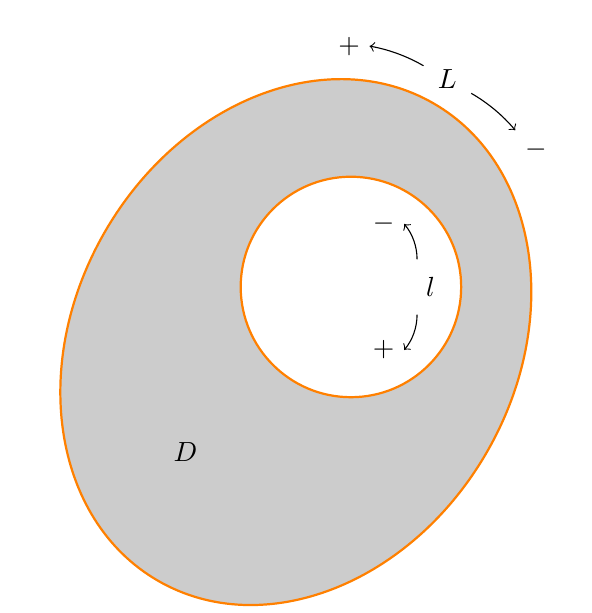
\begin{tikzpicture}[scale=.7]
	\draw[orange,fill=gray!40,rotate=60,thick] (0,0)ellipse[x radius=5,y radius=4];
	\draw[orange,fill=white,thick] (1,1)ellipse[x radius=2,y radius=2];
	\draw (-2,-2)node{\(D\)};
	\begin{scope}[rotate=60]
		\coordinate (P1) at (5.5,0);
		\draw (P1)node{\(L\)};
		\draw[->] (P1)+(0,.5) arc[start angle=0,end angle=20,radius=3]node[left]{\(+\)};
		\draw[->] (P1)+(0,-.5) arc[start angle=0,end angle=-20,radius=3]node[below right]{\(-\)};
	\end{scope}
	\begin{scope}
		\coordinate (P2) at (2.7,1);
		\draw (P2)node[left]{\(l\)};
		\draw[->] (P2)+(-.5,.5) arc[start angle=0,end angle=40,radius=1]node[left]{\(-\)};
		\draw[->] (P2)+(-.5,-.5) arc[start angle=0,end angle=-40,radius=1]node[left]{\(+\)};
	\end{scope}
\end{tikzpicture}
\caption{平面区域的边界曲线与其取向}
\label{figure:线积分与面积分.平面区域的边界曲线与其取向}
\end{figure}

\begin{theorem}[格林公式]
设闭区域\(D\)由分段光滑的曲线\(L\)围成,函数\(P(x,y)\)和\(Q(x,y)\)在\(D\)上具有一阶连续偏导数,则有
\begin{equation}\label{equation:线积分与面积分.格林公式}
\iint_D \left( \pdv{Q}{x} - \pdv{P}{y} \right) \dd{x}\dd{y}
= \oint_L P\dd{x} + Q\dd{y},
\end{equation}其中\(L\)是\(D\)的取正向的边界曲线.
\end{theorem}
\cref{equation:线积分与面积分.格林公式}叫做\DefineConcept{格林公式}.

下面说明格林公式的一个简单应用.
在格林公式中,令\(P=-y\)、\(Q=x\),可得\[
2 \iint_D \dd{x}\dd{y}
=\oint_L x\dd{y}-y\dd{x}.
\]上式左端是闭区域\(D\)的面积\(A\)的两倍,因此有
\begin{equation}\label{equation:线积分与面积分.利用格林公式计算闭区域的面积}
A = \frac{1}{2} \oint_L x\dd{y}-y\dd{x}.
\end{equation}
\begin{example}
求椭圆\(x = a \cos\theta, y = b \sin\theta\)所围成图形的面积\(A\).
\begin{solution}
根据\cref{equation:线积分与面积分.利用格林公式计算闭区域的面积} 有\begin{align*}
A &= \frac{1}{2} \oint_L x\dd{y}-y\dd{x} \\
&= \frac{1}{2} \int_0^{2\pi} \left[ a \cos\theta \cdot b \cos\theta \dd{\theta}
	- b \sin\theta \cdot (-a \sin\theta) \dd{\theta} \right] \\
&= \frac{1}{2} ab \int_0^{2\pi} \dd{\theta}
= \pi ab.
\end{align*}
\end{solution}
\end{example}

\begin{example}
计算\(\oint_L \frac{x\dd{y}-y\dd{x}}{x^2+y^2}\),其中\(L\)是一条不经过原点的分段光滑的若尔当闭曲线,\(L\)的方向为逆时针方向.
\begin{solution}
记\(P = -\frac{y}{x^2+y^2}, Q = \frac{x}{x^2+y^2}\).
当\(x^2+y^2\neq0\)时,有\[
\pdv{Q}{x} = \frac{y^2-x^2}{(x^2+y^2)^2} = \pdv{P}{y}.
\]记\(L\)所围成的闭区域为\(D\).

当\(\opair{0,0} \notin D\)时,由\cref{equation:线积分与面积分.格林公式} 有\[
\oint_L \frac{x\dd{y}-y\dd{x}}{x^2+y^2} = \iint_D 0 \dd{x}\dd{y} = 0;
\]

当\(\opair{0,0} \in D\)时,取\(r>0\)使得\(\Set{ \opair{x,y} \given x^2+y^2 \leqslant r^2 } \subseteq D\).作圆\(l: x^2+y^2=r^2\),记\(L\)和\(l\)所围成的闭区域为\(D_1\).
对复连通区域\(D_1\)应用格林公式,得\[
\oint_L \frac{x\dd{y}-y\dd{x}}{x^2+y^2} - \oint_l \frac{x\dd{y}-y\dd{x}}{x^2+y^2}
= \iint_{D_1} 0 \dd{x}\dd{y} = 0,
\]其中\(l\)的方向取逆时针方向.
于是\[
\oint_L \frac{x\dd{y}-y\dd{x}}{x^2+y^2}
= \oint_l \frac{x\dd{y}-y\dd{x}}{x^2+y^2}
= \int_0^{2\pi} \frac{r^2 \cos^2\theta + r^2 \sin^2\theta}{r^2} \dd{\theta}
= 2\pi.
\]
\end{solution}
\end{example}

\begin{example}[二维格林第一公式、二维格林第二公式]
设\(u(x,y)\)、\(v(x,y)\)在闭区域\(D\)上都具有二阶连续偏导数,分段光滑的曲线\(L\)为\(D\)的正向边界曲线.证明:\begin{gather}
\iint_D v \laplacian{u} \dd{x}\dd{y} = - \iint_D (\grad u \cdot \grad v) \dd{x}\dd{y} + \oint_L v \pdv{u}{\mat{n}} \dd{s};
\label{equation:线积分与面积分.二维格林第一公式} \\
\iint_D (u \laplacian v - v \laplacian u) \dd{x}\dd{y} = \oint_L \left( u \pdv{v}{\mat{n}} - v \pdv{u}{\mat{n}} \right) \dd{s},
\label{equation:线积分与面积分.二维格林第二公式}
\end{gather}其中\(\pdv{u}{\mat{n}}\)、\(\pdv{v}{\mat{n}}\)分别是\(u\)、\(v\)沿\(L\)的外法线向量\(\mat{n}\)的方向导数,二维拉普拉斯算子\(\laplacian = \pdv[2]{x} + \pdv[2]{y}\).
\begin{proof}
因为方向导数\[
\pdv{u}{\mat{n}}
= \pdv{u}{x} \cos\alpha
+ \pdv{u}{y} \cos\beta,
\qquad
\pdv{v}{\mat{n}}
= \pdv{v}{x} \cos\alpha
+ \pdv{v}{y} \cos\beta,
\]其中\(\cos\alpha\)、\(\cos\beta\)是\(L\)在点\(\opair{x,y}\)处的外法线向量的方向余弦,那么\(L\)在该点处的正向单位切向量为\(\mat{\tau} = \opair{-\cos\beta,\cos\alpha}\),于是利用格林公式可得\begin{align*}
\oint_L v \pdv{u}{\mat{n}} \dd{s}
&= \oint_L v \left(
\pdv{u}{x} \cos\alpha
+ \pdv{u}{y} \cos\beta
\right) \dd{s} \\
&= \oint_L \left( - v \pdv{u}{y} \right) \dd{x} + \left( v \pdv{u}{x} \right) \dd{y} \\
&= \iint_D \left[ \pdv{x} \left( v \pdv{u}{x} \right) - \pdv{y} \left( - v \pdv{u}{y} \right) \right] \dd{x}\dd{y} \\
&= \iint_D \left( \pdv{v}{x} \pdv{u}{x} + v \pdv[2]{u}{x} + \pdv{v}{y} \pdv{u}{y} + v \pdv[2]{u}{y} \right) \dd{x}\dd{y} \\
&= \iint_D (\grad u \cdot \grad v) \dd{x}\dd{y} + \iint_D v \laplacian{u} \dd{x}\dd{y},%
\end{align*}移项可得\cref{equation:线积分与面积分.二维格林第一公式}.而\cref{equation:线积分与面积分.二维格林第二公式} 可由\cref{equation:线积分与面积分.二维格林第一公式} 推得,故略去.
\end{proof}
\end{example}

\begin{example}
设函数\(f(x,y)\)在区域\(D=\Set{\opair{x,y} \given x^2+y^2\leqslant1}\)上具有二阶连续偏导数,且\(\pdv[2]{f}{x}+\pdv[2]{f}{y}=e^{-(x^2+y^2)}\),求二重积分\(I=\iint_D\left(x\pdv{f}{x}+y\pdv{f}{y}\right)\dd{x}\dd{y}\).
\begin{solution}
考虑区域\(D\)的形状,将积分\(I\)化为在极坐标系下的积分,令\(x=\rho\cos\theta, y=\rho\sin\theta\):\begin{align*}
I &= \int_0^1 \rho\dd{\rho} \int_0^{2\pi} \left(\rho\cos\theta\pdv{f}{x}+\rho\sin\theta\pdv{f}{y}\right) \dd{\theta} \\
&= \int_0^1 \rho\dd{\rho} \int_0^{2\pi} \left[\pdv{f}{x}\dd(\rho\sin\theta)-\pdv{f}{y}\dd(\rho\cos\theta)\right].
\end{align*}
考虑到\(\dd{x}=\dd(\rho\cos\theta), \dd{y}=\dd(\rho\sin\theta)\),所以\[
I = \int_0^1 \rho\dd{\rho} \oint_{L_{\rho}: x^2+y^2=\rho^2} \pdv{f}{x}\dd{y}-\pdv{f}{y}\dd{x}.
\]应用\hyperref[equation:线积分与面积分.格林公式]{格林公式},则有\begin{align*}
\oint_{L_{\rho}: x^2+y^2=\rho^2} \pdv{f}{x}\dd{y}-\pdv{f}{y}\dd{x}
&= \iint_{D_{\rho}: x^2+y^2\leqslant\rho^2} \left(\pdv[2]{f}{x}+\pdv[2]{f}{y}\right) \dd{\sigma} \\
&= \iint_{D_{\rho}: x^2+y^2\leqslant\rho^2} e^{-(x^2+y^2)} \dd{\sigma} \\
&= \int_0^{2\pi} \dd{\theta} \int_0^{\rho} e^{-\rho^2} \rho\dd{\rho} \\
&= \pi \left(1-e^{-\rho^2}\right).
\end{align*}
那么\[
I = \int_0^1 \pi \left(1-e^{-\rho^2}\right) \rho\dd{\rho}
=  \frac{\pi}{2e}.
\]
\end{solution}
\end{example}

\subsection{平面上曲线积分与路径无关的条件}
在物理上(特别是力学中)要研究所谓“势场”,就是要研究场力所作的功与路径无关的情形.
在什么条件下场力所作的功与路径无关?
这个问题在数学上就是要研究曲线积分与路径无关的条件.
为了研究这个问题,先要明确什么叫做“曲线积分\(\int_L P\dd{x}+Q\dd{y}\)与路径无关”.
\begin{definition}
设\(G\)是一个区域,\(P(x,y)\)以及\(Q(x,y)\)在区域\(G\)内具有一阶连续偏导数.
如果对于\(G\)内任意指定的两个点\(A\)、\(B\)
以及\(G\)内从点\(A\)到点\(B\)的任意两条曲线\(L_1\)、\(L_2\),%
等式\[
\int_{L_1}{P\dd{x}+Q\dd{y}}
=\int_{L_2}{P\dd{x}+Q\dd{y}}
\]恒成立,%
就说“曲线积分\(\int_L P\dd{x}+Q\dd{y}\)在\(G\)内与路径无关”,
否则便说“曲线积分\(\int_L P\dd{x}+Q\dd{y}\)在\(G\)内与路径相关”.
\end{definition}
“曲线积分\(\int_L P\dd{x}+Q\dd{y}\)在\(G\)内与路径无关”相当于“沿\(G\)内任意闭曲线\(C\)的曲线积分\(\oint_C P\dd{x}+Q\dd{y}\)等于零”.

\begin{theorem}\label{theorem:线积分与面积分.平面上曲线积分与路径无关的充要条件}
设区域\(G\)是一个单连通域,函数\(P(x,y)\)、\(Q(x,y)\)在\(G\)内具有一阶连续偏导数,那么曲线积分\(\int_L P\dd{x}+Q\dd{y}\)在\(G\)内与路径无关(或沿\(G\)内任意闭曲线的曲线积分为零)的充要条件是:\[
\pdv{P}{y}=\pdv{Q}{x}
\]在\(G\)内恒成立.
\end{theorem}
如果\cref{theorem:线积分与面积分.平面上曲线积分与路径无关的充要条件} 所要求的两个条件“区域\(G\)是单连通区域,且函数\(P(x,y)\)和\(Q(x,y)\)在\(G\)内具有一阶连续偏导数”不能同时满足,那么定理的结论不能保证成立.
例如当区域\(G\)中出现破坏函数\(P\)、\(Q\)及\(\pdv{Q}{x}\)、\(\pdv{P}{y}\)连续性条件的\DefineConcept{奇点}时,定理的结论就不能保证成立.

\subsection{二元函数的全微分求积}
\begin{theorem}\label{theorem:线积分与面积分.二元函数的全微分的存在条件}
设区域\(G\)是一个单连通区域.
函数\(P(x,y)\)、\(Q(x,y)\)在\(G\)内具有一阶连续偏导数.
则\(P(x,y)\dd{x}+Q(x,y)\dd{y}\)在\(G\)内为某一函数\(u(x,y)\)的全微分的充要条件是\[
\pdv{P}{y}=\pdv{Q}{x}
\]在\(G\)内恒成立.
\end{theorem}

根据\cref{theorem:线积分与面积分.平面上曲线积分与路径无关的充要条件} 和\cref{theorem:线积分与面积分.二元函数的全微分的存在条件},立即可得如下推论.
\begin{corollary}
设区域\(G\)是一个单连通区域.
函数\(P(x,y)\)、\(Q(x,y)\)在\(G\)内具有一阶连续偏导数.
则曲线积分\(\int_L{P\dd{x}+Q\dd{y}}\)在\(G\)内与路径无关的充要条件是:
在\(G\)内存在函数\(u(x,y)\),使\(\dd{u}=P\dd{x}+Q\dd{y}\).
\end{corollary}

\subsection{曲线积分的基本定理}
\begin{definition}
若曲线积分\(\int_L \mat{F}\cdot\dd{\mat{r}}\)在区域\(G\)内与积分路径无关,则称向量场\(\mat{F}\)为\DefineConcept{保守场}.
\end{definition}

下面的定理给出了平面曲线积分与路径无关的另一种形式的条件,并为计算保守场中的曲线积分提供了一种简便的方法.
\begin{theorem}[曲线积分的基本定理]\label{theorem:线积分与面积分.曲线积分的基本定理}
设\(\mat{F}(x,y)=P(x,y)\mat{i}+Q(x,y)\mat{j}\)是平面区域\(G\)内的一个向量场,%
\(P(x,y)\)、\(Q(x,y)\)都在\(G\)内连续,且存在一个数量函数\(f(x,y)\),%
使得\(\mat{F}=\grad{f}\),%
则曲线积分\(\int_L{\mat{F}\cdot\dd{\mat{r}}}\)在\(G\)内与路径无关,且
\begin{equation}\label{equation:线积分与面积分.曲线积分的基本公式}
\int_L \mat{F} \cdot \dd{\mat{r}}
= f(B)-f(A),
\end{equation}
其中\(L\)是位于\(G\)内起点为\(A\)、终点为\(B\)的任一分段光滑曲线.
\end{theorem}
\cref{theorem:线积分与面积分.曲线积分的基本定理} 表明,对于势场\(\mat{F}\),曲线积分\(\int_L \mat{F}\cdot\dd{\mat{r}}\)的值仅依赖于它的势函数\(f\)在路径\(L\)的两端点的值,而不依赖于两点间的路径,即积分\(\int_L \mat{F}\cdot\dd{\mat{r}}\)在\(G\)内与路径无关.
也就是说:势场是保守场.

\cref{equation:线积分与面积分.曲线积分的基本公式}
是与微积分基本公式\[
\int_a^b f(x) \dd{x}
= F(b) - F(a)
\](其中\(F'(x) = f(x)\))完全类似的向量微积分的相应公式,%
称为\DefineConcept{曲线积分的基本公式}.

\section{对面积的曲面积分}
\subsection{对面积的曲线积分的概念}
\begin{definition}
设曲面\footnote{以后都假定曲面的边界曲线是分段光滑的闭曲线,且曲面有界.}%
\(\Sigma\)是光滑的\footnote{如果曲面上各点处都具有切平面,则称该曲面是光滑的.
如果曲面是由有限个光滑曲面所组成的,则称该曲面是分片光滑的.}.
函数\(f(x,y,z)\)在\(\Sigma\)上有界.
把\(\Sigma\)任意分成\(n\)小块\(\increment S_i\)(\(\increment S_i\)同时也代表第\(i\)小块曲面的面积),设\(\opair{\xi_i,\eta_i,\zeta_i}\)是\(\increment S_i\)上任取的一点,作乘积\(f(\xi_i,\eta_i,\zeta_i) \increment S_i\ (i=1,2,\dotsc,n)\),并作和\(\sum\limits_{i=1}^n f(\xi_i,\eta_i,\zeta_i) \increment S_i\),如果当各小块曲面的直径\footnote{曲面的直径是指曲面上任意两点间距离的最大者.}的最大值\(\lambda\to0\)时,这和的极限总存在,则称此极限为函数\(f(x,y,z)\)在曲面\(\Sigma\)上\DefineConcept{对面积的曲面积分}或\DefineConcept{第一类曲面积分}(type I surface integral),记作\(\iint_{\Sigma}{f(x,y,z)\dd{S}}\),即\[
\iint_{\Sigma} f(x,y,z)\dd{S}
= \lim\limits_{\lambda\to0} \sum\limits_{i=1}^n f(\xi_i,\eta_i,\zeta_i) \increment S_i,
\]其中\(f(x,y,z)\)叫做\DefineConcept{被积函数},\(\Sigma\)叫做\DefineConcept{积分曲面}.

如果曲面\(\Sigma\)是分片光滑的,我们规定函数在\(\Sigma\)上对面积的曲面积分等于函数在光滑的各片曲面上对面积的曲面积分之和.
\end{definition}
我们指出,当被积函数\(f(x,y,z)\)在光滑曲面\(\Sigma\)上连续时,对面积的曲面积分是存在的.

\subsection{对面积的曲线积分的性质}
由对面积的曲面积分的定义可知,它具有与对弧长的曲线积分相类似的性质,这里不再赘述.

\subsection{对面积的曲面积分的计算法}
\begin{theorem}
设积分曲面\(\Sigma\)由方程\(z=z(x,y)\)给出,%
\(\Sigma\)在\(xOy\)面上的投影区域为\(D_{xy}\),%
函数\(z=z(x,y)\)在\(D_{xy}\)上具有连续偏导数,%
被积函数\(f(x,y,z)\)在\(\Sigma\)上连续.
那么有\[
\iint_{\Sigma}{f(x,y,z)\dd{S}}
=\iint_{D_{xy}}{f[x,y,z(x,y)] \sqrt{1+[z'_x(x,y)]^2+[z'_y(x,y)]^2} \dd{x}\dd{y}}.
\]
\end{theorem}
这就是把对面积的曲面积分化为二重积分的公式.
在计算时,只要把变量\(z\)换为\(z(x,y)\),\(\dd{S}\)换为\(\sqrt{1+(z'_x)^2+(z'_y)^2} \dd{x}\dd{y}\),再确定\(\Sigma\)在\(xOy\)面上的投影区域\(D_{xy}\),这样就把对面积的曲面积分化为二重积分了.

如果积分曲面\(\Sigma\)由方程\(x=x(y,z)\)或\(y=y(z,x)\)给出,也可类似地把对面积的曲面积分化为相应的二重积分.

可以将上述对面积的曲面积分的计算法总结为如下更一般的方法.
\begin{theorem}
设积分曲面\(\Sigma\)由二元向量值参数方程\[
\mat{r}(u,v) = x(u,v) \mat{i} + y(u,v) \mat{j} + z(u,v) \mat{k},
\quad \opair{u,v} \in D
\]给出,函数\(\mat{r}(u,v)\)在\(D\)上具有连续偏导数,%
被积函数\(f(x,y,z)\)在\(\Sigma\)上连续,那么有\[
\iint_{\Sigma} f(x,y,z) \dd{S}
= \iint_D f[\mat{r}(u,v)] \abs{\mat{r}'_u \times \mat{r}'_v} \dd{\sigma}.
\]
\end{theorem}
这里,参数\(u\)、\(v\)可以代换为\(x\)、\(y\)、\(z\)中任意两个,区域\(D\)可以代换为\(D_{xy}\)、\(D_{yz}\)或\(D_{zx}\).

\begin{example}
计算曲面积分\(\iint_{\Sigma} \frac{\dd{S}}{z}\),其中\(\Sigma\)是球面\(x^2+y^2+z^2=a^2\)被平面\(z = h\ (0<h<a)\)截出的顶部.
\begin{solution}
\(\Sigma\)的方程为\(z = \sqrt{a^2-x^2-y^2}\).
\(\Sigma\)在\(xOy\)面上的投影区域\(D_{xy}\)为圆形闭区域\[
\Set{\opair{x,y} \given x^2+y^2 \leqslant a^2-h^2}.
\]又\[
\sqrt{1+(z'_x)^2+(z'_y)^2} = \frac{a}{\sqrt{a^2-x^2-y^2}},
\]所以\[
\iint_{\Sigma} \frac{\dd{S}}{z}
= \iint_{D_{xy}} \frac{a\dd{x}\dd{y}}{a^2-x^2-y^2}.
\]利用极坐标,得\[
\iint_{\Sigma} \frac{\dd{S}}{z}
= \iint_{D_{xy}} \frac{a\rho\dd{\rho}\dd{\theta}}{a^2-\rho^2}
= a \int_0^{2\pi} \dd{\theta} \int_0^{\sqrt{a^2-h^2}} \frac{\rho\dd{\rho}}{a^2-\rho^2}
= 2\pi a \ln\frac{a}{h}.
\]
\end{solution}
\end{example}

\begin{example}
计算\(\varoiint_{\Sigma} xyz \dd{S}\),其中\(\Sigma\)是由平面\(x=0\)、\(y=0\)、\(z=0\)及\(x+y+z=1\)所围成的四面体的整个边界曲面.
\begin{solution}
整个边界曲面\(\Sigma\)在平面\(x=0\)、\(y=0\)、\(z=0\)及\(x+y+z=1\)上的部分依次记为\(\AutoTuple{\Sigma}{4}\),于是\[
\varoiint_{\Sigma} xyz \dd{S}
= \varoiint_{\Sigma_1} xyz \dd{S}
+ \varoiint_{\Sigma_2} xyz \dd{S}
+ \varoiint_{\Sigma_3} xyz \dd{S}
+ \varoiint_{\Sigma_4} xyz \dd{S}.
\]
由于在\(\AutoTuple{\Sigma}{3}\)上,被积函数\(f(x,y,z)=xyz\)均为零,所以\[
\varoiint_{\Sigma_1} xyz \dd{S}
= \varoiint_{\Sigma_2} xyz \dd{S}
= \varoiint_{\Sigma_3} xyz \dd{S}
= 0.
\]

在\(\Sigma_4\)上,\(z=1-x-y\),\(z'_x = z'_y = -1\),所以\[
\sqrt{1+(z'_x)^2+(z'_y)^2}
= \sqrt{1+(-1)^2+(-1)^2}
= \sqrt{3},
\]从而\[
\varoiint_{\Sigma} xyz \dd{S}
= \varoiint_{\Sigma_4} xyz \dd{S}
= \iint_{D_{xy}} \sqrt{3} xy (1-x-y) \dd{x} \dd{y},
\]其中\(D_{xy}\)是\(\Sigma_4\)在\(xOy\)面上的投影区域,即由直线\(x=0\)、\(y=0\)及\(x+y=1\)所围成的闭区域.
因此\[
\varoiint_{\Sigma} xyz \dd{S}
= \sqrt{3} \int_0^1 x \dd{x} \int_0^{1-x} y (1-x-y) \dd{y}
= \frac{\sqrt{3}}{120}.
\]
\end{solution}
\end{example}

\begin{example}
设点\(P\)是椭球面\(S: x^2 + y^2 + z^2 - yz = 1\)上的动点,若\(S\)在点\(P\)处的切平面与\(xOy\)面垂直,求点\(P\)的轨迹\(C\),并计算曲面积分\[
I = \iint_{\Sigma} \frac{(x+\sqrt{3}) \abs{y-2z}}{\sqrt{4+y^2+z^2-4yz}} \dd{S},
\]其中\(\Sigma\)是椭球面\(S\)位于曲线\(C\)上方的部分.
\begin{solution}
设\(F(x,y,z) = x^2 + y^2 + z^2 - yz - 1\).
求导得\[
F'_x = 2x, \qquad
F'_y = 2y - z, \qquad
F'_z = 2z - y,
\]那么\(S\)在点\(P\opair{x,y,z}\)处的切向量为\(\mat{n} = \opair{2x,2y-z,2z-y}\).
因为点\(P\)处的切平面与\(xOy\)面垂直,所以法向量\(\mat{n}\)与\(xOy\)面的法向量\(\opair{0,0,1}\)垂直,\[
2x\cdot0 + (2y-z)\cdot0+(2z-y)\cdot1=0
\quad\text{或}\quad
2z-y=0.
\]因此,轨迹\(C\)的方程是\[
\begin{cases}
x^2 + y^2 + z^2 - yz = 1, \\
2z-y=0.
\end{cases}
\]消去轨迹\(C\)方程中的\(z\),得到\(C\)在\(xOy\)面上的投影为\[
C_{xy}: x^2+\frac{3}{4}y^2=1.
\]又因为\[
z'_x = - \frac{F'_x}{F'_z} = \frac{2x}{y-2z}, \qquad
z'_y = - \frac{F'_y}{F'_z} = \frac{2y-z}{y-2z},
\]\begin{align*}
\dd{S} &= \sqrt{1+(z'_x)^2+(z'_y)^2} \dd{x}\dd{y} \\
&= \sqrt{1+\left(\frac{2x}{y-2z}\right)^2+\left(\frac{2y-z}{y-2z}\right)^2} \dd{x}\dd{y} \\
&= \frac{\sqrt{4x^2+5y^2+5z^2-8yz}}{\abs{y-2z}} \dd{x}\dd{y} \\
&= \frac{\sqrt{4+y^2+z^2-4yz}}{\abs{y-2z}} \dd{x}\dd{y},
\end{align*}所以\begin{align*}
&\hspace{-20pt}
\iint_{\Sigma} \frac{(x+\sqrt{3}) \abs{y-2z}}{\sqrt{4+y^2+z^2-4yz}} \dd{S} \\
&= \iint_{x^2+\frac{3}{4}y^2\leqslant1} \frac{(x+\sqrt{3}) \abs{y-2z}}{\sqrt{4+y^2+z^2-4yz}} \cdot \frac{\sqrt{4+y^2+z^2-4yz}}{\abs{y-2z}} \dd{x}\dd{y} \\
&= \iint_{x^2+\frac{3}{4}y^2\leqslant1} (x+\sqrt{3}) \dd{x}\dd{y} \\
&= \sqrt{3} \iint_{x^2+\frac{3}{4}y^2\leqslant1} \dd{x}\dd{y}
= 2\pi.
\end{align*}
\end{solution}
\end{example}

\subsection{利用对称性简化第一类曲面积分的计算}
设积分曲面\(\Sigma\)关于\(xOy\)面对称.
若被积函数\(f(x,y,z)\)是关于\(z\)的偶函数,即\(f(x,y,-z) = f(x,y,z)\),则\[
\iint_{\Sigma} f(x,y,z) \dd{S} = 2 \iint_{D_{xy}} f[x,y,z(x,y)] \sqrt{1+(z'_x)^2+(z'_y)^2} \dd{x}\dd{y};
\]若被积函数\(f(x,y,z)\)是关于\(z\)的奇函数,即\(f(x,y,-z) = -f(x,y,z)\),则\[
\iint_{\Sigma} f(x,y,z) \dd{S} = 0.
\]

类似地,可以得出,在积分曲面关于\(yOz\)面或\(zOx\)面对称,而被积函数\(f(x,y,z)\)是关于\(x\)或\(y\)的奇函数或偶函数的情形下,第一类曲面积分的简化计算公式.

\begin{example}
计算\(\varoiint_{\Sigma} x^2 \dd{S}\),其中\(\Sigma: x^2+y^2+z^2=a^2\).
\begin{solution}
利用对称性可得\begin{align*}
\varoiint_{\Sigma} x^2 \dd{S}
&= \frac{1}{3} \varoiint_{\Sigma} (x^2+y^2+z^2) \dd{S} \\
&= \frac{1}{3} \varoiint_{\Sigma} a^2 \dd{S}
= \frac{a^2}{3} \varoiint_{\Sigma} \dd{S} \\
&= \frac{a^2}{3} \cdot 4\pi a^2
= \frac{4}{3} \pi a^4.
\end{align*}
\end{solution}
\end{example}

\section{对坐标的曲面积分}
\subsection{对坐标的曲面积分的概念}
通常我们遇到的曲面都是双侧的.
例如由方程\(z = z(x,y)\)表示的曲面,有上侧与下侧之分\footnote{按惯例,这里假定\(z\)轴竖直向上.};又例如,一张包围某一空间区域的闭曲面,有外侧与内侧之分.
以后我们总假定所考虑的曲面是双侧的.

在讨论对坐标的曲面积分时,需要制定曲面的侧.
我们可以通过曲面上的法向量的指向来定出曲面的侧.
例如,对于曲面\(z = z(x,y)\),如果取它的法向量\(\mat{n}\)的指向朝上,我们就认为取定曲面的上侧;
又如,对于闭曲面如果取它的法向量的指向朝外,我们就认为取定曲面的外侧.
这种取定了法向量亦即选定了侧的曲面,就称为\DefineConcept{有向曲面}.

设\(\Sigma\)是有向曲面.
在\(\Sigma\)上取一小块曲面\(\increment S\),把\(\increment S\)投影到\(xOy\)面上得一投影区域,这投影区域的面积记为\((\increment\sigma)_{xy}\).
假定\(\increment S\)上各点处的法向量与\(z\)轴的夹角\(\gamma\)的余弦\(\cos\gamma\)有相同的符号(即\(\cos\gamma\)都是正的或都是负的).
我们规定\(\increment S\)在\(xOy\)面上的投影\((\increment S)_{xy}\)为\[
(\increment S)_{xy}
= \sgn\cos\gamma \cdot (\increment \sigma)_{xy}
= \left\{ \begin{array}{cc}
(\increment \sigma)_{xy}, & \cos\gamma > 0, \\
-(\increment \sigma)_{xy}, & \cos\gamma < 0, \\
0, & \cos\gamma \equiv 0.
\end{array} \right.
\]其中,\(\cos\gamma \equiv 0\)也就是\((\increment \sigma)_{xy} = 0\)的情形.
\(\increment S\)在\(xOy\)面上的投影\((\increment S)_{xy}\)实际就是\(\increment S\)在\(xOy\)面上的投影区域的面积附以一定的正负号.
类似地可以定义\(\increment S\)在\(yOz\)面及\(zOx\)面上的投影\((\increment S)_{yz}\)和\((\increment S)_{zx}\).

\begin{definition}
设\(\Sigma\)为光滑的有向曲面,函数\(R(x,y,z)\)在\(\Sigma\)上有界.
把\(\Sigma\)任意分成\(n\)块小曲面\(\increment S_i\)%
(\(\increment S_i\)同时又表示第\(i\)块小曲面的面积),%
\(\increment S_i\)在\(xOy\)面上的投影为\((\increment S_i)_{xy}\),%
\(\opair{\xi_i,\eta_i,\zeta_i}\)是\(\increment S_i\)上任意取定的一点.
如果当各小块曲面的直径的最大值\(\lambda\to0\)时,极限\[
\lim\limits_{\lambda\to0} \sum\limits_{i=1}^n R(\xi_i,\eta_i,\zeta_i) (\increment S_i)_{xy}
\]总存在,则称此极限为“函数\(R(x,y,z)\)在有向曲面\(\Sigma\)上对坐标\(x\)、\(y\)的\DefineConcept{曲面积分}”,%
记作\[\iint_{\Sigma} R(x,y,z) \dd{x}\dd{y},\]即\[
\iint_{\Sigma} R(x,y,z) \dd{x}\dd{y}
=\lim\limits_{\lambda\to0} \sum\limits_{i=1}^n R(\xi_i,\eta_i,\zeta_i) (\increment S_i)_{xy},
\]其中\(R(x,y,z)\)叫做\DefineConcept{被积函数},\(\Sigma\)叫做\DefineConcept{积分曲面}.

类似地可以定义%
“函数\(P(x,y,z)\)在有向曲面\(\Sigma\)上对坐标\(y\)、\(z\)的\DefineConcept{曲面积分}”\[\iint_{\Sigma} P(x,y,z) \dd{y}\dd{z}\]
及%
“函数\(Q(x,y,z)\)在有向曲面\(\Sigma\)上对坐标\(z\)、\(x\)的\DefineConcept{曲面积分}”\[\iint_{\Sigma} Q(x,y,z) \dd{z}\dd{x}\]
分别为
\begin{gather*}
\iint_{\Sigma} P(x,y,z) \dd{y}\dd{z}
	\defeq \lim\limits_{\lambda\to0} \sum\limits_{i=1}^n P(\xi_i,\eta_i,\zeta_i) (\increment S_i)_{yz}, \\
\iint_{\Sigma} Q(x,y,z) \dd{z}\dd{x}
	\defeq \lim\limits_{\lambda\to0} \sum\limits_{i=1}^n Q(\xi_i,\eta_i,\zeta_i) (\increment S_i)_{zx}.
\end{gather*}

以上三个曲面积分也称为\DefineConcept{第二类曲面积分}(type II surface integral).

如果\(\Sigma\)是分片光滑的有向曲面,我们规定函数在\(\Sigma\)上对坐标的曲面积分等于函数在各片光滑曲面上对坐标的曲面积分之和.
\end{definition}

我们指出,当\(P(x,y,z),Q(x,y,z),R(x,y,z)\)在有向光滑曲面\(\Sigma\)上连续时,对坐标的曲面积分是存在的.

一般地,可以将\[
\iint_{\Sigma} P(x,y,z) \dd{y}\dd{z}
+\iint_{\Sigma} Q(x,y,z) \dd{z}\dd{x}
+\iint_{\Sigma} R(x,y,z) \dd{x}\dd{y}
\]合并写成\[
\iint_{\Sigma}{P(x,y,z)\dd{y}\dd{z}+Q(x,y,z)\dd{z}\dd{x}+R(x,y,z)\dd{x}\dd{y}}.
\]

\subsection{对坐标的曲面积分的性质}
对坐标的曲面积分具有与对坐标的曲线积分相类似的一些性质.
\begin{property}
如果把\(\Sigma\)分成\(\Sigma_1\)和\(\Sigma_2\),则\begin{align*}
&\iint_{\Sigma}{P\dd{y}\dd{z}+Q\dd{z}\dd{x}+R\dd{x}\dd{y}} \\
&\qquad=\iint_{\Sigma_1}{P\dd{y}\dd{z}+Q\dd{z}\dd{x}+R\dd{x}\dd{y}} \\
&\qquad\quad+\iint_{\Sigma_2}{P\dd{y}\dd{z}+Q\dd{z}\dd{x}+R\dd{x}\dd{y}}.
\end{align*}
\end{property}

\begin{property}
设\(\Sigma\)是有向曲面,\(\Sigma^-\)表示与\(\Sigma\)取相反侧的有向曲面,则\begin{gather*}
\iint_{\Sigma^-} P(x,y,z) \dd{y}\dd{z} = -\iint_{\Sigma} P(x,y,z) \dd{y}\dd{z}, \\
\iint_{\Sigma^-} Q(x,y,z) \dd{z}\dd{x} = -\iint_{\Sigma} Q(x,y,z) \dd{z}\dd{x}, \\
\iint_{\Sigma^-} R(x,y,z) \dd{x}\dd{y} = -\iint_{\Sigma} R(x,y,z) \dd{x}\dd{y}.
\end{gather*}
\end{property}

\subsection{对坐标的曲面积分的计算法}
\begin{theorem}
设被积函数\(P(x,y,z)\)、\(Q(x,y,z)\)和\(R(x,y,z)\)在\(\Sigma\)上连续.
又设积分曲面\(\Sigma\)的单位法向量为\(\mat{n} = \opair{\cos\alpha,\cos\beta,\cos\gamma}\).

如果\(\Sigma\)由\(z=z(x,y)\)给出,%
且\(z=z(x,y)\)在\(D_{xy}\)上具有一阶连续偏导数,%
则有\begin{equation}\label{equation:线积分与面积分.第二类曲面积分的计算式1}
\iint_{\Sigma} R(x,y,z) \dd{x}\dd{y}
= \sgn\cos\gamma \cdot \iint_{D_{xy}} R[x,y,z(x,y)] \dd{x}\dd{y}.
\end{equation}
\(\sgn\cos\gamma\)的取值可以这样判定 —— 当积分曲面为\(\Sigma\)上侧时,上式等号右侧取正号;当积分曲面为\(\Sigma\)下侧时,上式等号右侧取负号.

如果\(\Sigma\)由\(y=y(z,x)\)给出,%
且\(y=y(z,x)\)在\(D_{zx}\)上具有一阶连续偏导数,%
则有\begin{equation}\label{equation:线积分与面积分.第二类曲面积分的计算式2}
\iint_{\Sigma} Q(x,y,z) \dd{z}\dd{x}
= \sgn\cos\beta \cdot \iint_{D_{zx}} Q[x,y(z,x),z] \dd{z}\dd{x}.
\end{equation}
\(\sgn\cos\beta\)的取值可以这样判定 —— 当积分曲面为\(\Sigma\)右侧时,上式等号右侧取正号;当积分曲面为\(\Sigma\)左侧时,上式等号右侧取负号.

如果\(\Sigma\)由\(x=x(y,z)\)给出,%
且\(x=x(y,z)\)在\(D_{yz}\)上具有一阶连续偏导数,%
则有\begin{equation}\label{equation:线积分与面积分.第二类曲面积分的计算式3}
\iint_{\Sigma} P(x,y,z) \dd{y}\dd{z}
= \sgn\cos\alpha \cdot \iint_{D_{yz}} P[x(y,z),y,z] \dd{y}\dd{z}.
\end{equation}
\(\sgn\cos\alpha\)的取值可以这样判定 —— 当积分曲面为\(\Sigma\)前侧时,上式等号右侧取正号;当积分曲面为\(\Sigma\)后侧时,上式等号右侧取负号.
\end{theorem}

可以将上述对坐标的曲面积分的计算法总结为如下更一般的方法.
\begin{theorem}
设积分曲面\(\Sigma\)由二元向量值参数方程\[
\mat{r}(u,v) = x(u,v) \mat{i} + y(u,v) \mat{j} + z(u,v) \mat{k},
\quad \opair{u,v} \in D
\]给出,这里\(D\)是\(uv\)平面上具有分段光滑边界的有界闭区域,%
且\(\mat{r}\colon D \to \Sigma\)是具有一阶连续偏导数的单值函数,%
且雅克比矩阵\[
\mat{J} = \begin{bmatrix}
x'_u & x'_v \\
y'_u & y'_v \\
z'_u & z'_v
\end{bmatrix}
\]是满秩的,%
且被积函数\[
\mat{F}(x,y,z) = P(x,y,z) \mat{i} + Q(x,y,z) \mat{j} + R(x,y,z) \mat{k}
\]在\(\Sigma\)上连续,那么有\[
\iint_{\Sigma} \mat{F} \cdot \dd{\mat{S}}
= \pm \iint_D \left[
	P \jacobi{y,z}{u,v}
	+ Q \jacobi{z,x}{u,v}
	+ R \jacobi{x,y}{u,v}
\right] \dd{u}\dd{u}.
\]
\end{theorem}

\begin{example}
计算曲面积分\[
\iint_{\Sigma} x^2 \dd{y}\dd{z} + y^2 \dd{z}\dd{x} + z^2 \dd{x}\dd{y},
\]其中\(\Sigma\)是长方体\(\Omega = \Set{
\opair{x,y,z} \given
0 \leqslant x \leqslant a,
0 \leqslant y \leqslant b,
0 \leqslant z \leqslant c
}\)的整个表面的外侧.
\begin{solution}
把有向曲面\(\Sigma\)分成以下六部分:
\begin{center}\begin{tabular}{l}
\(\Sigma_1: z=c\ (0 \leqslant x \leqslant a, 0 \leqslant y \leqslant b)\)的上侧; \\
\(\Sigma_2: z=0\ (0 \leqslant x \leqslant a, 0 \leqslant y \leqslant b)\)的下侧; \\
\(\Sigma_3: x=a\ (0 \leqslant y \leqslant b, 0 \leqslant z \leqslant c)\)的前侧; \\
\(\Sigma_4: x=0\ (0 \leqslant y \leqslant b, 0 \leqslant z \leqslant c)\)的后侧; \\
\(\Sigma_5: y=b\ (0 \leqslant x \leqslant a, 0 \leqslant z \leqslant c)\)的右侧; \\
\(\Sigma_6: y=0\ (0 \leqslant x \leqslant a, 0 \leqslant z \leqslant c)\)的左侧. \\
\end{tabular}\end{center}
除\(\Sigma_3\)、\(\Sigma_4\)外,其余四片曲面在\(yOz\)面上的投影为零,因此\[
\iint_{\Sigma} x^2 \dd{y}\dd{z}
= \iint_{\Sigma_3} x^2 \dd{y}\dd{z}
+ \iint_{\Sigma_4} x^2 \dd{y}\dd{z}.
\]应用\cref{equation:线积分与面积分.第二类曲面积分的计算式3} 就有\[
\iint_{\Sigma} x^2 \dd{y}\dd{z}
= \iint_{D_{yz}} a^2 \dd{y}\dd{z}
- \iint_{D_{yz}} 0^2 \dd{y}\dd{z}
= a^2 bc.
\]同理可得\[
\iint_{\Sigma} y^2 \dd{z}\dd{x}
= b^2 ac,
\]\[
\iint_{\Sigma} z^2 \dd{x}\dd{y}
= c^2 ab.
\]于是所求曲面积分为\((a+b+c) abc\).
\end{solution}
\end{example}

\begin{example}
计算曲面积分\(\iint_{\Sigma} xyz \dd{x}\dd{y}\),其中\(\Sigma\)是球面\(x^2+y^2+z^2=1\)外侧在\(x\geqslant0,y\geqslant0\)的部分.
\begin{solution}
把\(\Sigma\)分为\(\Sigma_1\)和\(\Sigma_2\)两部分,其中\(\Sigma_1\)的方程为\[
z = -\sqrt{1-x^2-y^2},
\]而\(\Sigma_2\)的方程为\[
z = \sqrt{1-x^2-y^2}.
\]因此\begin{align*}
\iint_{\Sigma} xyz \dd{x}\dd{y}
&= \iint_{\Sigma_1} xyz \dd{x}\dd{y}
+ \iint_{\Sigma_2} xyz \dd{x}\dd{y} \\
&= -\iint_{D_{xy}} xy (-\sqrt{1-x^2-y^2}) \dd{x}\dd{y}
+ \iint_{D_{xy}} xy \sqrt{1-x^2-y^2} \dd{x}\dd{y} \\
&= 2 \iint_{D_{xy}} xy \sqrt{1-x^2-y^2} \dd{x}\dd{y}.
\end{align*}
其中\(D_{xy}\)是\(\Sigma_1,\Sigma_2\)在\(xOy\)面上的投影区域,就是位于第一象限内的扇形\[
x^2+y^2\leqslant1 \quad(x\geqslant0,y\geqslant0).
\]利用极坐标计算这个二重积分如下:\begin{align*}
2 \iint_{D_{xy}} xy \sqrt{1-x^2-y^2} \dd{x}\dd{y}
&= 2 \iint_{D_{xy}} \rho^2 \sin\theta \cos\theta \sqrt{1-\rho^2} \rho\dd{\rho}\dd{\theta} \\
&= \int_0^{\pi/2} \sin2\theta \dd{\theta} \int_0^1 \rho^3 \sqrt{1-\rho^2} \dd{\rho} \\
&= 1 \cdot \frac{2}{15} = \frac{2}{15},
\end{align*}
从而\(\iint_{\Sigma} xyz \dd{x}\dd{y} = \frac{2}{15}\).
\end{solution}
\end{example}

\subsection{利用对称性简化第二类曲面积分的计算}
设积分曲面\(\Sigma\)关于\(xOy\)面对称.
若被积函数\(f(x,y,z)\)是关于\(z\)的偶函数,即\[
	f(x,y,-z) = f(x,y,z),
\]
则\[
	\iint_{\Sigma} f(x,y,z) \dd{x}\dd{y} = 0;
\]
若被积函数\(f(x,y,z)\)是关于\(z\)的奇函数,即\[
	f(x,y,-z) = -f(x,y,z),
\]
则\[
	\iint_{\Sigma} f(x,y,z) \dd{x}\dd{y} = \pm2 \iint_{D_{xy}} f[x,y,z(x,y)] \dd{x}\dd{y}.
\]

类似地,可以得出,在积分曲面关于\(yOz\)面或\(zOx\)面对称,
而被积函数\(f(x,y,z)\)是关于\(x\)或\(y\)的奇函数或偶函数的情形下,
第二类曲面积分的简化计算公式.

\section{两类曲面积分之间的联系}
设有向曲面\(\Sigma\)由方程\(z = z(x,y)\)给出,\(\Sigma\)在\(xOy\)面上的投影区域为\(D_{xy}\),函数\(z = z(x,y)\)在\(D_{xy}\)上具有一阶连续偏导数,\(R(x,y,z)\)在\(\Sigma\)上连续.
如果\(\Sigma\)取上侧,则由对坐标的曲面积分计算公式有\[
\iint_{\Sigma} R(x,y,z) \dd{x}\dd{y} = \iint_{D_{xy}} R[x,y,z(x,y)] \dd{x}\dd{y}.
\]

另一方面,因上述有向曲面\(\Sigma\)的法向量的方向余弦为\[
\cos\alpha=\frac{-z'_x}{\sqrt{1+(z'_x)^2+(z'_y)^2}},
\]\[
\cos\beta=\frac{-z'_y}{\sqrt{1+(z'_x)^2+(z'_y)^2}},
\]\[
\cos\gamma=\frac{1}{\sqrt{1+(z'_x)^2+(z'_y)^2}},
\]故由对面积的曲面积分计算公式有\[
\iint_{\Sigma} R(x,y,z) \cos\gamma \dd{S}
= \iint_{D_{xy}} R[x,y,z(x,y)] \dd{x}\dd{y}.
\]由此可见,有\[
\iint_{\Sigma} R(x,y,z) \dd{x}\dd{y}
= \iint_{\Sigma} R(x,y,z) \cos\gamma \dd{S}.
\eqno{(1)}
\]

如果\(\Sigma\)取下侧,则\[
\iint_{\Sigma} R(x,y,z) \cos\gamma \dd{S}
= -\iint_{D_{xy}} R[x,y,z(x,y)] \dd{x}\dd{y}.
\]但这时\(\cos\gamma=\frac{-1}{\sqrt{1+(z'_x)^2+(z'_y)^2}}\),因此(1)式仍成立.

类似地可推得\[
\iint_{\Sigma} P(x,y,z) \dd{y}\dd{z}
= \iint_{D_{yz}} P(x,y,z) \cos\alpha \dd{S},
\eqno{(2)}
\]\[
\iint_{\Sigma} Q(x,y,z) \dd{z}\dd{x}
= \iint_{D_{zx}} Q(x,y,z) \cos\beta \dd{S}.
\eqno{(3)}
\]

合并(1)、(2)、(3)式,得两类曲面积分之间的如下联系:
\begin{equation}\label{equation:线积分与面积分.两类曲面积分之间的联系}
\iint_{\Sigma} P \dd{y}\dd{z} + Q \dd{z}\dd{x} + R \dd{x}\dd{y}
=\iint_{\Sigma} (P\cos\alpha+Q\cos\beta+R\cos\gamma) \dd{S},
\end{equation}
其中\(\cos\alpha\)、\(\cos\beta\)、\(\cos\gamma\)是有向曲面\(\Sigma\)在点\(\opair{x,y,z}\)处的法向量的方向余弦.

两类曲面积分之间的联系也可写成如下的向量形式:
\begin{equation}\label{equation:线积分与面积分.两类曲面积分之间的联系的向量形式}
\iint_{\Sigma} \mat{A} \cdot \dd{\mat{S}}
=\iint_{\Sigma} \mat{A} \cdot \mat{n} \dd{S},
\end{equation}
其中\(\mat{A}=\opair{P,Q,R}\),%
\(\mat{n}=\opair{\cos\alpha,\cos\beta,\cos\gamma}\)为有向曲面\(\Sigma\)在点\(\opair{x,y,z}\)处的单位法向量,%
\(\dd{\mat{S}} = \mat{n}\dd{S} = \opair{\dd{y}\dd{z},\dd{z}\dd{x},\dd{x}\dd{y}}\)称为\DefineConcept{有向曲面元}.

\begin{example}
\def\ys{\iint_{\Sigma} (z^2+x) \dd{y}\dd{z} - z \dd{x}\dd{y}}%
计算曲面积分\(\ys\),其中\(\Sigma\)是旋转抛物面\(z = \frac{1}{2}(x^2+y^2)\)介于平面\(z=0\)和\(z=2\)之间的部分的下侧.
\begin{solution}
由两类曲面积分之间的联系 \labelcref{equation:线积分与面积分.两类曲面积分之间的联系},可得\[
\iint_{\Sigma} (z^2+x) \dd{y}\dd{z}
= \iint_{\Sigma} (z^2+x) \cos\alpha \dd{S}
= \iint_{\Sigma} (z^2+x) \frac{\cos\alpha}{\cos\gamma} \dd{x}\dd{y}.
\]在曲面\(\Sigma\)上,有\[
\cos\alpha
= \frac{x}{\sqrt{1+x^2+y^2}},
\qquad
\cos\gamma
= \frac{-1}{\sqrt{1+x^2+y^2}}.
\]故\[
\ys
= \iint_{\Sigma} [(z^2+x)(-x) - z] \dd{x}\dd{y}.
\]
再按对坐标的曲面积分的计算法,便得\[
\ys
= - \iint_{D_{xy}} \left\{
	\left[
		\frac{1}{4} (x^2+y^2)^2
		+ x
	\right] \cdot (-x)
	- \frac{1}{2} (x^2+y^2)
\right\} \dd{x}\dd{y}.
\]因为\(\iint_{D_{xy}} \frac{1}{4} x(x^2+y^2)^2 \dd{x}\dd{y} = 0\),所以\begin{align*}
\ys
&= \iint_{D_{xy}} \left[x^2+\frac{1}{2}(x^2+y^2)\right] \dd{x}\dd{y} \\
&= \int_0^{2\pi} \dd{\theta} \int_0^2 \left(\rho^2 \cos^2\theta + \frac{1}{2} \rho^2\right) \rho \dd{\rho}
= 8\pi.
\end{align*}
\end{solution}
\end{example}

\section{高斯公式,通量与散度}
\subsection{高斯公式}
格林公式表达了平面闭区域上的二重积分与其边界曲线上的曲线积分之间的关系,
而高斯公式表达了空间闭区域上的三重积分与其边界曲面上的曲面积分之间的关系,
这个关系可以陈述如下:
\begin{theorem}
设空间闭区域\(\Omega\)是由分片光滑的闭曲面\(\Sigma\)所围成;
在\(\Omega\)上,函数\(P,Q,R\)都具有一阶连续偏导数,则有
\begin{equation}\label{equation:线积分与面积分.高斯公式}
	\begin{split}
		\iiint_{\Omega} \left(\pdv{P}{x}+\pdv{Q}{y}+\pdv{R}{z}\right)\dd{v}
		&=\varoiint_{\Sigma} P\dd{y}\dd{z}+Q\dd{z}\dd{x}+R\dd{x}\dd{y} \\
		&=\varoiint_{\Sigma} (P\cos\alpha+Q\cos\beta+R\cos\gamma)\dd{S},
	\end{split}
\end{equation}
这里\(\Sigma\)是\(\Omega\)的整个边界曲面的外侧,
\(\cos\alpha,\cos\beta,\cos\gamma\)是\(\Sigma\)在点\(\opair{x,y,z}\)处的法向量的方向余弦.

\rm\cref{equation:线积分与面积分.高斯公式} 叫做\DefineConcept{高斯公式}.
\begin{proof}
设闭区域\(\Omega\)在\(xOy\)面上的投影区域为\(D_{xy}\).
假定穿过\(\Omega\)内部且平行于\(z\)轴的直线与\(\Omega\)的边界曲面\(\Sigma\)的交点恰好是两个.
这样就可以将\(\Sigma\)分为\(\AutoTuple{\Sigma}{3}\)三部分,%
其中\(\Sigma_1\)、\(\Sigma_2\)分别由方程\(z=z_1(x,y)\)、\(z=z_2(x,y)\)给定,%
这里\(z_1(x,y) \leqslant z_2(x,y)\),%
\(\Sigma_1\)取下侧,\(\Sigma_2\)取上侧;
\(\Sigma_3\)是以\(D_{xy}\)的边界曲线为准线、母线平行于\(z\)轴的柱面上的一部分,取外侧.

根据三重积分的计算法,有\[\begin{aligned}
\iiint_{\Omega} \pdv{R}{z} \dd{v}
&= \iint_{D_{xy}} \left[
	\int_{z_1(x,y)}^{z_2(x,y)} \pdv{R}{z} \dd{z}
\right] \dd{x}\dd{y} \\
&= \iint_{D_{xy}} \left\{
	R[x,y,z_2(x,y)] - R[x,y,z_1(x,y)]
\right\} \dd{x}\dd{y}.
\end{aligned}
\eqno{(1)}
\]
根据曲面积分的计算法,有\[
\iint_{\Sigma_1} R(x,y,z) \dd{x}\dd{y}
= -\iint_{D_{xy}} R[x,y,z_1(x,y)] \dd{x}\dd{y}.
\]\[
\iint_{\Sigma_2} R(x,y,z) \dd{x}\dd{y}
= \iint_{D_{xy}} R[x,y,z_2(x,y)] \dd{x}\dd{y}.
\]因为\(\Sigma_3\)上任意一块曲面在\(xOy\)面上的投影为零,所以直接根据对坐标的曲面积分的定义可知\[
\iint_{\Sigma_3} R(x,y,z) \dd{x}\dd{y} = 0.
\]把以上三个式子相加,得\[
\varoiint_{\Sigma} R(x,y,z) \dd{x}\dd{y}
= \iint_{D_{xy}} \left\{
	R[x,y,z_2(x,y)] - R[x,y,z_1(x,y)]
\right\} \dd{x}\dd{y}.
\eqno{(2)}
\]比较(1)、(2)两式,得\[
\iiint_{\Omega} \pdv{R}{z} \dd{v} = \varoiint_{\Sigma} R(x,y,z) \dd{x}\dd{y}.
\]

如果穿过\(\Omega\)内部且平行于\(x\)轴的直线以及平行于\(y\)轴的直线与\(\Omega\)的边界曲面\(\Sigma\)的交点也都恰好是两个,那么类似地可得\[
\iiint_{\Omega} \pdv{P}{x} \dd{v} = \varoiint_{\Sigma} P(x,y,z) \dd{y}\dd{z},
\]\[
\iiint_{\Omega} \pdv{Q}{y} \dd{v} = \varoiint_{\Sigma} Q(x,y,z) \dd{z}\dd{x},
\]再把以上三个式子两端分别相加,即得高斯公式 \labelcref{equation:线积分与面积分.高斯公式}.

在上述证明中,我们对闭区域\(\Omega\)作了这样的限制,即穿过\(\Omega\)内部且平行于坐标轴的直线与\(\Omega\)的边界曲面\(\Sigma\)的交点恰好是两点.
如果\(\Omega\)不满足这样的条件,可以引进几张辅助曲面,把\(\Omega\)分为有限个闭区域,使得每个闭区域满足这样的条件,并注意到沿辅助曲面相反两侧的两个曲面积分的绝对值相等而符号相反,相加时正好抵消,因此\cref{equation:线积分与面积分.高斯公式} 对于这样的闭区域仍然是正确的.
\end{proof}
\end{theorem}


\begin{example}
利用高斯公式计算曲面积分\[
\varoiint_{\Sigma} (x-y) \dd{x}\dd{y} + (y-z)x \dd{y}\dd{z},
\]其中\(\Sigma\)为柱面\(x^2+y^2=1\)及平面\(z=0,z=3\)所围成的空间闭区域\(\Omega\)的整个边界曲面的外侧.
\begin{solution}
记\(P=(y-z)x\),\(Q=0\),\(R=x-y\),那么\[
\pdv{P}{x} = y-z,
\qquad
\pdv{Q}{y} = 0,
\qquad
\pdv{R}{z} = 0,
\]利用高斯公式把所给曲面积分化为三重积分,再利用柱面坐标计算三重积分,得\begin{align*}
&\hspace{-20pt}\varoiint_{\Sigma} (x-y) \dd{x}\dd{y} + (y-z)x \dd{y}\dd{z}
= \iiint_{\Omega} (y-z) \dd{x}\dd{y}\dd{z} \\
&= \iiint_{\Omega} (\rho\sin\theta-z)\rho\dd{\rho}\dd{\theta}\dd{z}
= \int_0^{2\pi} \dd{\theta} \int_0^1 \rho\dd{\rho} \int_0^3 (\rho\sin\theta-z) \dd{z}
= -\frac{9\pi}{2}.
\end{align*}
\end{solution}
\end{example}

\begin{example}
设空间有界区域\(\Omega\)中,柱面\(x^2+y^2=1\)与平面\(z=0\)和\(x+z=1\)围成,\(\Sigma\)为\(\Omega\)边界曲面的外侧,计算曲面积分\[
I = \varoiint_{\Sigma} 2xz \dd{y}\dd{z} + xz \cos y \dd{z}\dd{x} + 3yz \sin x \dd{x}\dd{y}.
\]
\begin{solution}
利用高斯公式可得
\begin{align*}
I &= \iiint_{\Omega} \left[ \pdv{x}(2xz) + \pdv{y}(xz \cos y) + \pdv{z}(3yz \sin x) \right] \dd{v} \\
&= \iiint_{\Omega} (2z - xz \sin y + 3y \sin x) \dd{v}.
\end{align*}
注意到积分区域\(\Omega\)关于\(xOz\)面对称,那么\[
\iiint_{\Omega} xz \sin y \dd{v} = 0,
\qquad
\iiint_{\Omega} 3y \sin x \dd{v} = 0;
\]因此\begin{align*}
I &= 2 \iiint_{\Omega} z \dd{x}\dd{y}\dd{z}
= 2 \iint_{D_{xy}} \dd{x}\dd{y} \int_0^{1-x} z \dd{z} \\
&= \iint_{D_{xy}} (1-x)^2 \dd{x}\dd{y}
= \iint_{D_{xy}} (1-2x+x^2) \dd{x}\dd{y} \\
&= \iint_{D_{xy}} \dd{x}\dd{y}
- 2 \iint_{D_{xy}} x \dd{x}\dd{y}
+ \iint_{D_{xy}} x^2 \dd{x}\dd{y},
\end{align*}
其中\(D_{xy} = \Set{\opair{x,y} \given x^2+y^2\leqslant1}\).
注意到\(\iint_{D_{xy}} \dd{x}\dd{y}\)是区域\(D_{xy}\)的面积,取值为\(\pi\cdot1^2=\pi\);
又有\(\iint_{D_{xy}} x \dd{x}\dd{y}\)中积分区域\(D_{xy}\)关于\(x\)轴对称,且被积函数\(x\)是奇函数,那么\(\iint_{D_{xy}} x \dd{x}\dd{y} = 0\);
同时,由于\(D_{xy}\)关于原点对称,\[
\iint_{D_{xy}} x^2 \dd{x}\dd{y} = \iint_{D_{xy}} y^2 \dd{x}\dd{y},
\]所以\begin{align*}
I &= \pi + \frac{1}{2} \iint_{D_{xy}} (x^2+y^2) \dd{x}\dd{y} \\
&= \pi + \frac{1}{2}
	\int_0^{2\pi} \dd{\theta} \int_0^1 \rho^2 \cdot \rho\dd{\rho}
= \frac{5}{4} \pi.
\end{align*}
\end{solution}
\end{example}

\begin{example}[三维格林第一公式]
设函数\(u(x,y,z)\)和\(v(x,y,z)\)在闭区域\(\Omega\)上具有一阶及二阶连续偏导数,\(\Sigma\)是闭区域\(\Omega\)的整个边界曲面,\(\pdv{v}{\mat{n}}\)为函数\(v(x,y,z)\)沿\(\Sigma\)的外法线方向的方向导数.证明:
\begin{equation}\label{equation:线积分与面积分.三维格林第一公式}
\begin{split}
&\iiint_{\Omega} u \laplacian{v} \dd{x}\dd{y}\dd{z} \\
&\hspace{30pt}=\varoiint_{\Sigma} u \pdv{v}{n} \dd{S}
-\iiint_{\Omega} \left(
\pdv{u}{x} \pdv{v}{x}
+\pdv{u}{y} \pdv{v}{y}
+\pdv{u}{z} \pdv{v}{z}
\right) \dd{x}\dd{y}\dd{z},
\end{split}
\end{equation}其中符号\(\laplacian = \pdv[2]{x} + \pdv[2]{y} + \pdv[2]{z}\)为\DefineConcept{拉普拉斯算子}.
\begin{proof}
因为方向导数\[
\pdv{v}{\mat{n}}
= \pdv{v}{x} \cos\alpha
+ \pdv{v}{y} \cos\beta
+ \pdv{v}{z} \cos\gamma,
\]其中\(\cos\alpha\)、\(\cos\beta\)、\(\cos\gamma\)是\(\Sigma\)在点\(\opair{x,y,z}\)处的外法线向量的方向余弦,于是利用高斯公式即有曲面积分\begin{align*}
&\hspace{-20pt}\varoiint_{\Sigma} u \pdv{v}{\mat{n}} \dd{S}
= \varoiint_{\Sigma} u \left(
\pdv{v}{x} \cos\alpha
+ \pdv{v}{y} \cos\beta
+ \pdv{v}{z} \cos\gamma
\right) \dd{S} \\
&= \varoiint_{\Sigma} \left[
\left( u \pdv{v}{x} \right) \cos\alpha
+ \left( u \pdv{v}{y} \right) \cos\beta
+ \left( u \pdv{v}{z} \right) \cos\gamma
\right] \dd{S} \\
&= \varoiint_{\Sigma} \left[
\pdv{x} \left( u \pdv{v}{x} \right)
+ \pdv{y} \left( u \pdv{v}{y} \right)
+ \pdv{z} \left( u \pdv{v}{z} \right)
\right] \dd{x}\dd{y}\dd{z} \\
&= \varoiint_{\Sigma} \left[
\left( \pdv{u}{x} \pdv{v}{x} + u \pdv[2]{v}{x} \right)
+ \left( \pdv{u}{y} \pdv{v}{y} + u \pdv[2]{v}{y} \right)
+ \left( \pdv{u}{z} \pdv{v}{z} + u \pdv[2]{v}{z} \right)
\right] \dd{x}\dd{y}\dd{z} \\
&= \varoiint_{\Sigma} \left(
\pdv{u}{x} \pdv{v}{x}
+ \pdv{u}{y} \pdv{v}{y}
+ \pdv{u}{z} \pdv{v}{z}
\right) \dd{x}\dd{y}\dd{z}
+ \varoiint_{\Sigma} u \laplacian{v} \dd{x}\dd{y}\dd{z},
\end{align*}将上式右端第一个积分移至左端便得\cref{equation:线积分与面积分.三维格林第一公式}.
\end{proof}
\end{example}
\begin{example}[三维格林第二公式]
设函数\(u(x,y,z)\)和\(v(x,y,z)\)在闭区域\(\Omega\)上具有二阶连续偏导数,\(\Sigma\)是闭区域\(\Omega\)的整个边界曲面,\(\pdv{u}{\mat{n}}\)、\(\pdv{v}{\mat{n}}\)依次为函数\(u\)、\(v\)沿\(\Sigma\)的外法线方向的方向导数.证明:
\begin{equation}\label{equation:线积分与面积分.三维格林第二公式}
\iiint_{\Omega} (u \laplacian{v} - v \laplacian{u}) \dd{x}\dd{y}\dd{z}
=\varoiint_{\Sigma} \left( u \pdv{v}{\mat{n}} - v \pdv{u}{\mat{n}} \right) \dd{S}.
\end{equation}
\begin{proof}
\def\Io{\iiint_{\Omega} \left(%
\pdv{u}{x} \pdv{v}{x}%
+\pdv{u}{y} \pdv{v}{y}%
+\pdv{u}{z} \pdv{v}{z}%
\right) \dd{x}\dd{y}\dd{z}}%
因为方向导数\begin{align*}
\pdv{u}{\mat{n}}
&= \pdv{u}{x} \cos\alpha
+ \pdv{u}{y} \cos\beta
+ \pdv{u}{z} \cos\gamma, \\
\pdv{v}{\mat{n}}
&= \pdv{v}{x} \cos\alpha
+ \pdv{v}{y} \cos\beta
+ \pdv{v}{z} \cos\gamma,
\end{align*}其中\(\cos\alpha\)、\(\cos\beta\)、\(\cos\gamma\)是\(\Sigma\)在点\(\opair{x,y,z}\)处的外法线向量的方向余弦,于是利用\hyperref[equation:线积分与面积分.三维格林第一公式]{三维格林第一公式}即有曲面积分\begin{align*}
&\hspace{-5pt}\varoiint_{\Sigma} \left( u \pdv{v}{\mat{n}} - v \pdv{u}{\mat{n}} \right) \dd{S}
= \varoiint_{\Sigma} u \pdv{v}{\mat{n}} \dd{S}
- \varoiint_{\Sigma} v \pdv{u}{\mat{n}} \dd{S} \\
&= \left[ \iiint_{\Omega} u \laplacian{v} \dd{x}\dd{y}\dd{z} + I \right]
- \left[ \iiint_{\Omega} v \laplacian{u} \dd{x}\dd{y}\dd{z} + I \right] \\
&= \iiint_{\Omega} (u \laplacian{v} - v \laplacian{u}) \dd{x}\dd{y}\dd{z},
\end{align*}其中\(I = \Io\).
\end{proof}
\end{example}

\subsection{沿任意闭曲面的曲面积分为零的条件}
\begin{definition}
对于空间区域\(G\),如果\(G\)内任一闭曲面所围成的区域全属于\(G\),则称\(G\)是\DefineConcept{空间二维单连通区域};如果\(G\)内任一闭曲线总可以张成一片完全属于\(G\)的曲面,则称\(G\)为\DefineConcept{空间一维单连通区域}.
\end{definition}

\begin{example}
球面所围成的区域既是空间二维单连通的,又是空间一维单连通的.
环面所围成的区域是空间二维单连通的,但不是空间一维单连通的.
两个同心球面之间的区域是空间一维单连通的,但不是空间二维单连通的.
\end{example}

\begin{theorem}\label{theorem:线积分与面积分.沿任意闭曲面的曲面积分为零的条件}
设\(G\)是空间二维单连通区域,\(P(x,y,z)\)、\(Q(x,y,z)\)、\(R(x,y,z)\)在\(G\)内具有一阶连续偏导数,则曲面积分\[
\iint_{\Sigma} P\dd{y}\dd{z}+Q\dd{z}\dd{x}+R\dd{x}\dd{y}
\]在\(G\)内与所取曲面\(\Sigma\)无关而只决定于\(\Sigma\)的边界曲线(或沿\(G\)内任一闭曲面的曲面积分为零)的充要条件是\[
\pdv{P}{x}+\pdv{Q}{y}+\pdv{R}{z} = 0
\]在\(G\)内恒成立.
\end{theorem}

\subsection{通量与散度}
\begin{definition}
设有向量场\[
\mat{A}(x,y,z)=P(x,y,z)\mat{i}+Q(x,y,z)\mat{j}+R(x,y,z)\mat{k},
\]其中函数\(P\)、\(Q\)、\(R\)均具有一阶连续偏导数,\(\Sigma\)是场内一片有向曲面,\(\mat{n}\)是\(\Sigma\)在点\(\opair{x,y,z}\)处的单位法向量,则积分\[
\iint_{\Sigma}{\mat{A}\cdot\mat{n}\dd{S}}
\]称为向量场\(\mat{A}\)通过曲面\(\Sigma\)向着指定侧的\DefineConcept{通量}(或\DefineConcept{流量}).
\end{definition}
由两类曲面积分的关系,通量又可表达为\[
\iint_{\Sigma} \mat{A}\cdot\mat{n}\dd{S}
=\iint_{\Sigma} \mat{A}\cdot\dd{\mat{S}}
=\iint_{\Sigma} P\dd{y}\dd{z}+Q\dd{z}\dd{x}+R\dd{x}\dd{y}.
\]

\begin{definition}[平面上的散度]
\def\defofdiv{\lim\limits_{D \to M} \frac{1}{S} \oint_C \mat{A}(x,y) \cdot \dd{\mat{s}}}%
设\[
\mat{A}(x,y)=P(x,y)\mat{i}+Q(x,y)\mat{j}
\]是定义在平面闭区域\(D\)内的向量场,%
\(C\)是\(D\)的边界曲线的正向,%
\(D\)的面积\(S = \iint_{D} \dd{\sigma}\).
对于\(D\)内一点\(M\),称极限\[
\defofdiv
\]为向量场\(\mat{A}\)在点\(M\)的(二维)\DefineConcept{散度}(或\DefineConcept{通量密度}),记作\(\div{\mat{A}}\)或\(\operatorname{div}\mat{A}\),即\[
\div{\mat{A}} = \defofdiv.
\]
\end{definition}

\begin{theorem}
向量场\(\mat{A}(x,y)=P(x,y)\mat{i}+Q(x,y)\mat{j}\)的在点\(\opair{x,y}\)的散度为\[
\div{\mat{A}} = \pdv{P}{x}+\pdv{Q}{y}.
\]
\end{theorem}

\begin{definition}[空间中的散度]
\def\defofdiv{\lim\limits_{\Omega \to M} \frac{1}{V} \varoiint_{\Sigma} \mat{A}(x,y,z) \cdot \dd{\mat{S}}}%
设\[
\mat{A}(x,y,z)=P(x,y,z)\mat{i}+Q(x,y,z)\mat{j}+R(x,y,z)\mat{k}
\]是定义在空间闭区域\(\Omega\)内的向量场,%
\(\Sigma\)是\(\Omega\)的边界曲面的外侧,%
\(\Omega\)的体积\(V = \iiint_{\Omega} \dd{v}\).
对于\(\Omega\)内一点\(M\),称极限\[
\defofdiv
\]为向量场\(\mat{A}\)在点\(M\)的(三维)\DefineConcept{散度}(或\DefineConcept{通量密度}),记作\(\div{\mat{A}}\)或\(\operatorname{div}\mat{A}\),即\[
\div{\mat{A}} = \defofdiv.
\]
\end{definition}

\begin{theorem}
向量场\(\mat{A}(x,y,z)=P(x,y,z)\mat{i}+Q(x,y,z)\mat{j}+R(x,y,z)\mat{k}\)的在点\(\opair{x,y,z}\)的散度为\[
\div{\mat{A}} = \pdv{P}{x}+\pdv{Q}{y}+\pdv{R}{z}.
\]
\end{theorem}

\begin{definition}
若在点\(M\)处\(\div{\mat{A}}>0\),则称点\(M\)为向量场\(\mat{A}\)的\DefineConcept{源}(或\DefineConcept{正源});%
若在点\(M\)处\(\div{\mat{A}}<0\),则称点\(M\)为向量场\(\mat{A}\)的\DefineConcept{漏}(或\DefineConcept{负源});%
若在点\(M\)处\(\div{\mat{A}}=0\),则称向量场\(\mat{A}\)在点\(M\)处\DefineConcept{无源}.

如果向量场\(\mat{A}\)的散度\(\div{\mat{A}}\)处处为零,则称向量场\(\mat{A}\)为\DefineConcept{无源场}.
\end{definition}

现在利用散度的概念,\cref{equation:线积分与面积分.高斯公式} 可以改写为
\begin{equation}\label{equation:线积分与面积分.高斯公式1}
	\iiint_{\Omega} \div{\mat{A}} \dd{v} = \varoiint_{\Sigma} \mat{A} \cdot \dd{\mat{S}};
\end{equation}
而\cref{theorem:线积分与面积分.沿任意闭曲面的曲面积分为零的条件}
可以改写为“沿任意闭曲面的曲面积分为零的充要条件是向量场散度为零”.

\begin{example}
利用高斯公式推证阿基米德原理:浸没在液体中的物体所受液体的压力的合力(即浮力)的方向铅直向上,其大小等于这物体所排开的液体的重力.
\begin{proof}
我们建立如下的坐标系:\(xOy\)面与液面重合,\(z\)轴铅锤向下.
浸没在液体中的物体所占据的空间闭区域\(\Omega\)的边界曲面\(\Sigma\)上任意一点\(M\opair{x,y,z}\)的邻近小区域\(\dd{\sigma}\)所受的压力大小等于从它到液面间这部分液体(柱)的重力大小,即为\(\rho g z \dd{\sigma}\),而方向是\(\mat{n}=\cos\alpha\mat{i}+\cos\beta\mat{j}+\cos\gamma\mat{k}\)(即\(\Sigma\)的单位内法向量),其中\(\rho\)是液体的密度,\(\sigma\)是液体(柱)的底面积,\(g\)是重力加速度大小.
从而整个物体所受浮力为\begin{align*}
\mat{F} &= \varoiint_{\Sigma} \rho g z (\cos\alpha\mat{i}+\cos\beta\mat{j}+\cos\gamma\mat{k}) \dd{\sigma} \\
&= \rho g \iint_{\Omega} \left(\pdv{x}+\pdv{y}+\pdv{z}\right) z \dd{v} \\
&= \rho g \iint_{\Omega} \dd{v}
= \rho g V,
\end{align*}其中\(V\)是物体所排开的液体的体积.
\end{proof}
\end{example}

\section{斯托克斯公式 环流量与旋度}
\subsection{斯托克斯公式}
斯托克斯公式是\hyperref[equation:线积分与面积分.格林公式]{格林公式}的推广.格林公式表达了平面闭区域上的二重积分与其边界曲线上的曲线积分间的关系,而斯托克斯公式则把曲面\(\Sigma\)上的曲面积分与沿着\(\Sigma\)的边界曲线的曲线积分联系起来.这个联系可陈述如下:

\begin{theorem}[斯托克斯公式]
设\(\Gamma\)为分段光滑的空间有向闭曲线,%
\(\Sigma\)是以\(\Gamma\)为边界的分片光滑的有向曲面,%
\(\Gamma\)的正向与\(\Sigma\)的侧符合“右手规则%
\footnote{右手规则是指当右手除拇指外的四指依\(\Gamma\)的绕行方向时,%
拇指所指的方向与\(\Sigma\)上法向量的指向相同.
这时称\(\Gamma\)是有向曲面\(\Sigma\)的\DefineConcept{正向边界曲线}.}”,%
函数\(P(x,y,z)\)、\(Q(x,y,z)\)、\(R(x,y,z)\)在曲面\(\Sigma\)(连同边界\(\Gamma\))上具有一阶连续偏导数,则有
\begin{equation}\label{equation:线积分与面积分.斯托克斯公式}
\begin{split}
&\hspace{-20pt}\iint_{\Sigma}
	\left( \pdv{R}{y} - \pdv{Q}{z} \right)\dd{y}\dd{z}
	+\left( \pdv{P}{z} - \pdv{R}{x} \right)\dd{z}\dd{x}
	+\left( \pdv{Q}{x} - \pdv{P}{y} \right)\dd{x}\dd{y} \\
&= \oint_{\Gamma} P\dd{x}+Q\dd{y}+R\dd{z}.
\end{split}
\end{equation}
\end{theorem}

为了便于记忆,利用行列式记号把斯托克斯公式写成\[
\iint_{\Sigma} \begin{vmatrix}
\dd{y}\dd{z} & \dd{z}\dd{x} & \dd{x}\dd{y} \\
\pdv{x} & \pdv{y} & \pdv{z} \\
P & Q & R \\
\end{vmatrix}
= \oint_{\Gamma} P\dd{x}+Q\dd{y}+R\dd{z},
\]把其中的行列式按第一行展开,并把\(\pdv{y}\)与\(R\)的“积”理解为\(\pdv{R}{y}\),并以此类推.

利用两类曲面积分间的联系,可得斯托克斯公式的另一形式\[
\iint_{\Sigma} \begin{vmatrix}
\cos\alpha & \cos\beta & \cos\gamma \\
\pdv{x} & \pdv{y} & \pdv{z} \\
P & Q & R \\
\end{vmatrix} \dd{S}
= \oint_{\Gamma} P\dd{x}+Q\dd{y}+R\dd{z},
\]其中\(\mat{n}=\opair{\cos\alpha,\cos\beta,\cos\gamma}\)为有向曲面\(\Sigma\)在点\(\opair{x,y,z}\)处的单位法向量.

如果我们再进一步借用分块矩阵的记法,则可将斯托克斯公式写成\[
\iint_{\Sigma} \begin{vmatrix}
\dd{\mat{S}} \\
\grad \\
\mat{A}
\end{vmatrix}
= \oint_{\Gamma} \mat{A} \cdot \dd{\mat{r}}
\quad\text{或}\quad
\iint_{\Sigma} \begin{vmatrix}
\mat{n} \\
\grad \\
\mat{A}
\end{vmatrix} \dd{S}
= \oint_{\Gamma} \mat{A} \cdot \dd{\mat{r}}.
\]

如果\(\Sigma\)是\(xOy\)面上的一块平面闭区域,斯托克斯公式就变成格林公式.因此,格林公式是斯托克斯公式的一种特殊情形,即\[
\iint_{\Sigma} \begin{vmatrix}
0 & 0 & \dd{x}\dd{y} \\
\pdv{x} & \pdv{y} & \pdv{z} \\
P & Q & 0 \\
\end{vmatrix}
= \oint_{\Gamma} P\dd{x}+Q\dd{y}.
\]

\subsection{空间曲线积分与路径无关的条件}
\begin{theorem}\label{theorem:线积分与面积分.空间曲线积分与路径无关的条件}
设空间区域\(G\)是一维单连通区域,函数\(P(x,y,z)\)、\(Q(x,y,z)\)、\(R(x,y,z)\)在\(G\)内具有一阶连续偏导数,则空间曲线积分\(\int_{\Gamma}{P\dd{x}+Q\dd{y}+R\dd{z}}\)在\(G\)内与路径无关(或沿\(G\)内任意闭曲线的曲线积分为零)的充要条件是\[
\pdv{P}{y}=\pdv{Q}{x}, \qquad
\pdv{Q}{z}=\pdv{R}{y}, \qquad
\pdv{R}{x}=\pdv{P}{z}
\]在\(G\)内恒成立.
\end{theorem}

\begin{theorem}
设区域\(G\)是空间一维单连通区域,%
函数\(P(x,y,z)\)、\(Q(x,y,z)\)、\(R(x,y,z)\)在\(G\)内具有一阶连续偏导数,%
则表达式\(P\dd{x}+Q\dd{y}+R\dd{z}\)在\(G\)内成为某一函数\(u(x,y,z)\)的全微分,即\begin{align*}
u(x,y,z)
&= \int_{\opair{x_0,y_0,z_0}}^{\opair{x,y,z}}
 P\dd{x}+Q\dd{y}+R\dd{z} \\
&= \int_{x_0}^x P(x,y_0,z_0) \dd{x}
+ \int_{y_0}^y Q(x,y,z_0) \dd{y}
+ \int_{z_0}^z R(x,y,z) \dd{z}
\end{align*}的充要条件是\[
\pdv{P}{y}=\pdv{Q}{x}, \qquad
\pdv{Q}{z}=\pdv{R}{y}, \qquad
\pdv{R}{x}=\pdv{P}{z}
\]在\(G\)内恒成立.
\end{theorem}

\subsection{环流量与旋度}
\begin{definition}
设有向量场\[
\mat{A}(x,y,z)=P(x,y,z)\mat{i}+Q(x,y,z)\mat{j}+R(x,y,z)\mat{k},
\]其中函数\(P\)、\(Q\)、\(R\)均连续,\(\Gamma\)是\(\mat{A}\)的定义域内的一条分段光滑的有向闭曲线,\(\mat{\tau}\)是\(\Gamma\)在点\(\opair{x,y,z}\)处的单位切向量,则积分\[
\oint_{\Gamma}{\mat{A}\cdot\mat{\tau}\dd{s}}
\]称为向量场\(\mat{A}\)沿有向闭曲线\(\Gamma\)的\DefineConcept{环流量}.
\end{definition}
由两类曲线积分的关系,环流量又可表达为\[
\oint_{\Gamma}{\mat{A}\cdot\mat{\tau}\dd{s}}
=\oint_{\Gamma}{\mat{A}\cdot\dd{\mat{r}}}
=\oint_{\Gamma}{P\dd{x}+Q\dd{y}+R\dd{z}}.
\]

\begin{definition}
设有向量场\[
\mat{A}(x,y,z)=P(x,y,z)\mat{i}+Q(x,y,z)\mat{j}+R(x,y,z)\mat{k},
\]其中函数\(P\)、\(Q\)、\(R\)均具有一阶连续偏导数,则向量\[
\left( \pdv{R}{y} - \pdv{Q}{z} \right)\mat{i}
+\left( \pdv{P}{z} - \pdv{R}{x} \right)\mat{j}
+\left( \pdv{Q}{x} - \pdv{P}{y} \right)\mat{k}
\]称为向量场\(\mat{A}\)的\DefineConcept{旋度},记作\(\curl{\mat{A}}\)或\(\operatorname{rot}\mat{A}\),即\[
\curl{\mat{A}}
=\left( \pdv{R}{y} - \pdv{Q}{z} \right)\mat{i}
+\left( \pdv{P}{z} - \pdv{R}{x} \right)\mat{j}
+\left( \pdv{Q}{x} - \pdv{P}{y} \right)\mat{k}.
\]
\end{definition}

为了便于记忆,利用行列式记号把旋度公式改写为\[
\curl{\mat{A}}
=\begin{vmatrix}
\mat{i} & \mat{j} & \mat{k} \\
\pdv{x} & \pdv{y} & \pdv{z} \\
P & Q & R \\
\end{vmatrix},
\]把其中的行列式按第一行展开,并把\(\pdv{y}\)与\(R\)的“积”理解为\(\pdv{R}{y}\),并以此类推.

\begin{definition}
如果向量场\(\mat{A}\)的旋度\(\curl{\mat{A}}\)处处为零,则称向量场\(\mat{A}\)为\DefineConcept{无旋场}.一个无源、无旋的向量场称为\DefineConcept{调和场}.
\end{definition}
调和场是物理学中一类重要的向量场,这种场与调和函数有密切的关系.

设斯托克斯公式中有向曲面\(\Sigma\)在点\(\opair{x,y,z}\)处的单位法向量为\[
\mat{n} = \cos\alpha \mat{i} + \cos\beta \mat{j} + \cos\gamma \mat{k},
\]则\[
(\curl{\mat{A}}) \cdot \mat{n} = \begin{vmatrix}
\cos\alpha & \cos\beta & \cos\gamma \\
\pdv{x} & \pdv{y} & \pdv{z} \\
P & Q & R \\
\end{vmatrix}.
\]于是,斯托克斯公式可以写成下面的向量形式\[
\iint_{\Sigma} \curl{\mat{A}} \cdot \mat{n} \dd{S} = \oint_L \mat{A} \cdot \mat{\tau} \dd{s}
\]或\[
\iint_{\Sigma} \curl{\mat{A}} \cdot \dd{\mat{S}} = \oint_L \mat{A} \cdot \dd{\mat{s}}.
\]上式表明:向量场\(\mat{A}\)沿有向闭曲线\(\Gamma\)的环流量等于向量场\(\mat{A}\)的旋度通过曲面\(\Sigma\)的通量,这里\(\Gamma\)的正向与\(\Sigma\)的侧应符合右手规则.

\begin{example}
证明:\(\curl(\mat{a}+\mat{b}) = \curl\mat{a} + \curl\mat{b}\).
\begin{proof}
因为\[
\curl\mat{a} = \begin{vmatrix}
\mat{i} & \mat{j} & \mat{k} \\
\pdv{x} & \pdv{y} & \pdv{z} \\
P_1 & Q_1 & R_1
\end{vmatrix},
\qquad
\curl\mat{b} = \begin{vmatrix}
\mat{i} & \mat{j} & \mat{k} \\
\pdv{x} & \pdv{y} & \pdv{z} \\
P_2 & Q_2 & R_2
\end{vmatrix},
\]所以\begin{align*}
\curl\mat{a} + \curl\mat{b}
&= \begin{vmatrix}
\mat{i} & \mat{j} & \mat{k} \\
\pdv{x} & \pdv{y} & \pdv{z} \\
P_1 & Q_1 & R_1
\end{vmatrix} + \begin{vmatrix}
\mat{i} & \mat{j} & \mat{k} \\
\pdv{x} & \pdv{y} & \pdv{z} \\
P_2 & Q_2 & R_2
\end{vmatrix} \\
&= \begin{vmatrix}
\mat{i} & \mat{j} & \mat{k} \\
\pdv{x} & \pdv{y} & \pdv{z} \\
P_1 + P_2 & Q_1 + Q_2 & R_1 + R_2
\end{vmatrix} \\
&= \curl(\mat{a}+\mat{b}). \qedhere
\end{align*}
\end{proof}
\end{example}

\begin{example}
设\(u = u(x,y,z)\)具有二阶连续偏导数,求\(\curl(\grad u)\).
\begin{solution}
因为\[
\grad u = \pdv{u}{x} \mat{i} + \pdv{u}{y} \mat{j} + \pdv{u}{z} \mat{k},
\]所以\[
\curl(\grad u)
= \left( \pdv[2]{u}{z}{y} - \pdv[2]{u}{y}{z} \right) \mat{i}
+ \left( \pdv[2]{u}{x}{z} - \pdv[2]{u}{z}{x} \right) \mat{j}
+ \left( \pdv[2]{u}{y}{x} - \pdv[2]{u}{x}{y} \right) \mat{k}.
\]又因为\(u(x,y,z)\)的二阶偏导数是连续的,那么\[
\pdv[2]{u}{z}{y} = \pdv[2]{u}{y}{z},
\qquad
\pdv[2]{u}{x}{z} = \pdv[2]{u}{z}{x},
\qquad
\pdv[2]{u}{y}{x} = \pdv[2]{u}{x}{y},
\]因此\(\curl(\grad u) = \mat{0}\).
\end{solution}
\end{example}
